\documentclass[a4paper,11pt]{report}
\usepackage[T1]{fontenc}
\usepackage[utf8]{inputenc}
\usepackage{lmodern}
\usepackage[english]{babel}
\usepackage{amsfonts}
\usepackage{hyperref}
\usepackage{graphicx}
\usepackage{subcaption}
\usepackage{float}

\title{Technical report from 08/08/2014 to 15/08/2014}
\author{Rafael Reggiani Manzo}

\begin{document}

\maketitle
\tableofcontents

\chapter{Previous meeting}
  \section{What was presented}
  Last time when we met, I've showed the results that I've achieved on a mask obtained from a fibre tracking with the stopping criteria at angles higher than 60 degrees instead of 45 degrees and then cropped to a small region of interest.

  The results using clustering algorithms showed no visually meaningful results for this small region. But, on the other hand, a implementation of a segmentation algorithm was capable of segmenting the corner region of the region of interest.

  \section{Next steps}
  From this we agreed that the next steps would be to first produce the maps the three eigenvalues of the tensor ($\lambda_1$, $\lambda_2$, $\lambda_3$), apply the same segmentation algorithm, then apply it to the FA, MD, RD and TV maps.

  After that, produce a prototype that accordingly to difference between the eigenvectors in order to produce a threshold mask. This should be configurable with parameters that may vary from full isotropy to full anisotropy.

\chapter{Work done}
  All the work expected from the last meeting was done in time as expected.

  \section{Eigenvalues differences threshold}
    Every index that we can extract from a tensor is associated to it's eigenvalues or is a combination of them. So looking at them, instead to derived indexes like FA, should provide more information about the dataset.

    Since the eigenvalues will be object of various discussions ahead we shall clarify that we are referencing the three eigenvalues as $\lambda_1$, $\lambda_2$ and $\lambda_3$ in decreasing order.

    \subsection{Procedure}
    In more details, what we are looking for when trying to map uncertainty and certainty on a dataset, is the differences between those values. For example:

    \begin{itemize}
      \item $\lambda_1 - \lambda_2 = 1.0$ and $\lambda_1 - \lambda_3 = 1.0$ and $\lambda_2 - \lambda_3 = 0.0$ represent what we call full anisotropy or, as we will reference to it later, perfect anisotropy;
      \item similarly, $\lambda_1 - \lambda_2 = 0.0$ and $\lambda_1 - \lambda_3 = 0.0$ and $\lambda_2 - \lambda_3 = 0.0$ represent what we call full isotropy or, as we will reference to it later, perfect isotropy.
    \end{itemize}

    Those represent the two kinds of region we are pursuing to map: perfect anisotropy is the most certainty region; and perfect isotropy is the most uncertainty region.

    Given this concept, we must consider that both cases never happen in real datasets. So this brings us a relaxation by a parameter $0 \leq \epsilon \leq 1$ for the expressions previously mentioned:

    \newpage
    \begin{itemize}
      \item $1 - \epsilon \leq \lambda_1 - \lambda_2 \leq 1.0$ and $1 - \epsilon \leq \lambda_1 - \lambda_3 \leq 1.0$ and $0.0 \leq \lambda_2 - \lambda_3 \leq \epsilon$;
      \item $0.0 \leq \lambda_1 - \lambda_2 \leq \epsilon$ and $0.0 \leq \lambda_1 - \lambda_3 \leq \epsilon$ and $0.0 \leq \lambda_2 - \lambda_3 \leq \epsilon$.
    \end{itemize}

    Then, by increasing the $\epsilon$ step by step we may find a threshold for approximations of perfect anisotropy and isotropy.

    \subsection{Results}
      \subsubsection{Control experiments}
      The whole dataset considered for this experiments is:

      \begin{figure}[H]
        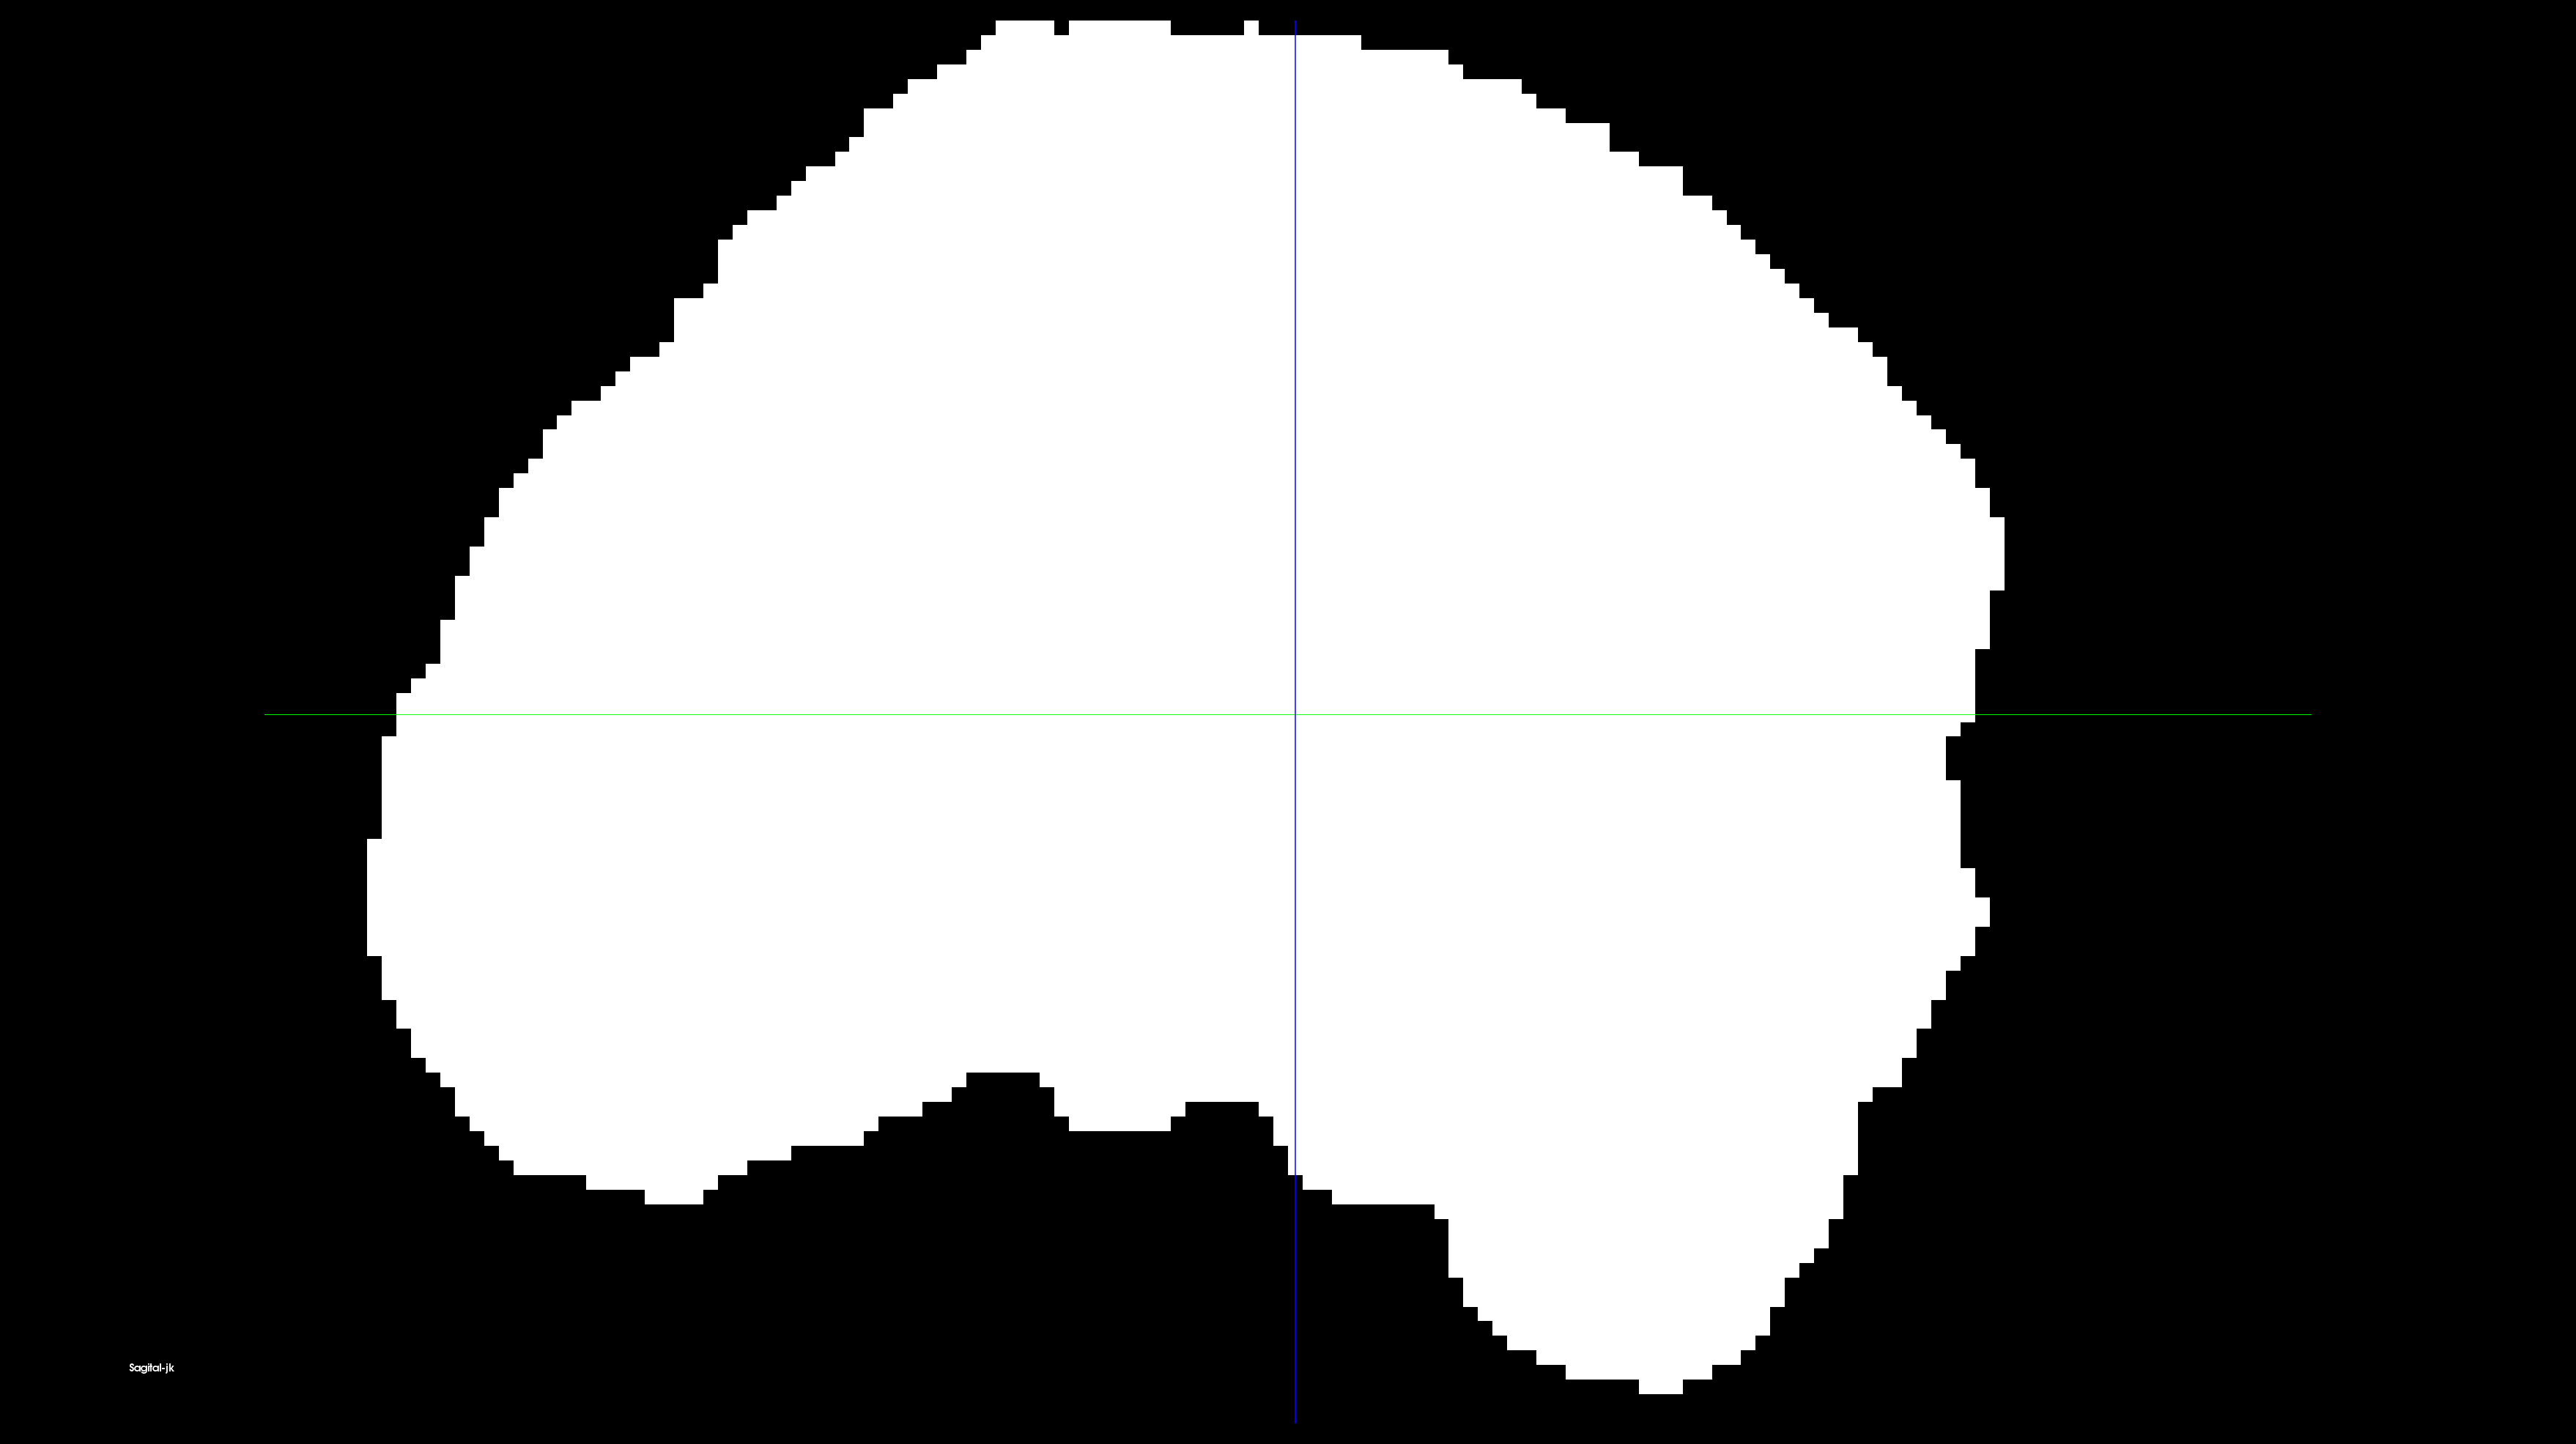
\includegraphics[width=1\linewidth]{imgs/whole.png}
        \caption{Sagital cut at (70, 70, 48) for the whole mask.}
        \label{fig:whole}
      \end{figure}

      This region has the following statistics:

      \begin{tabular}{| c | c | c |}
        \hline
        Number of voxels & FA mean & FA Standard Deviation \\ \hline
        460353 & 0.1964880 & 0.1662012 \\ \hline
      \end{tabular}

      .\newline

      For comparison purposes, lets first look at a simple FA threshold at 0.2 which should give us just the white matter:

      \begin{figure}[H]
        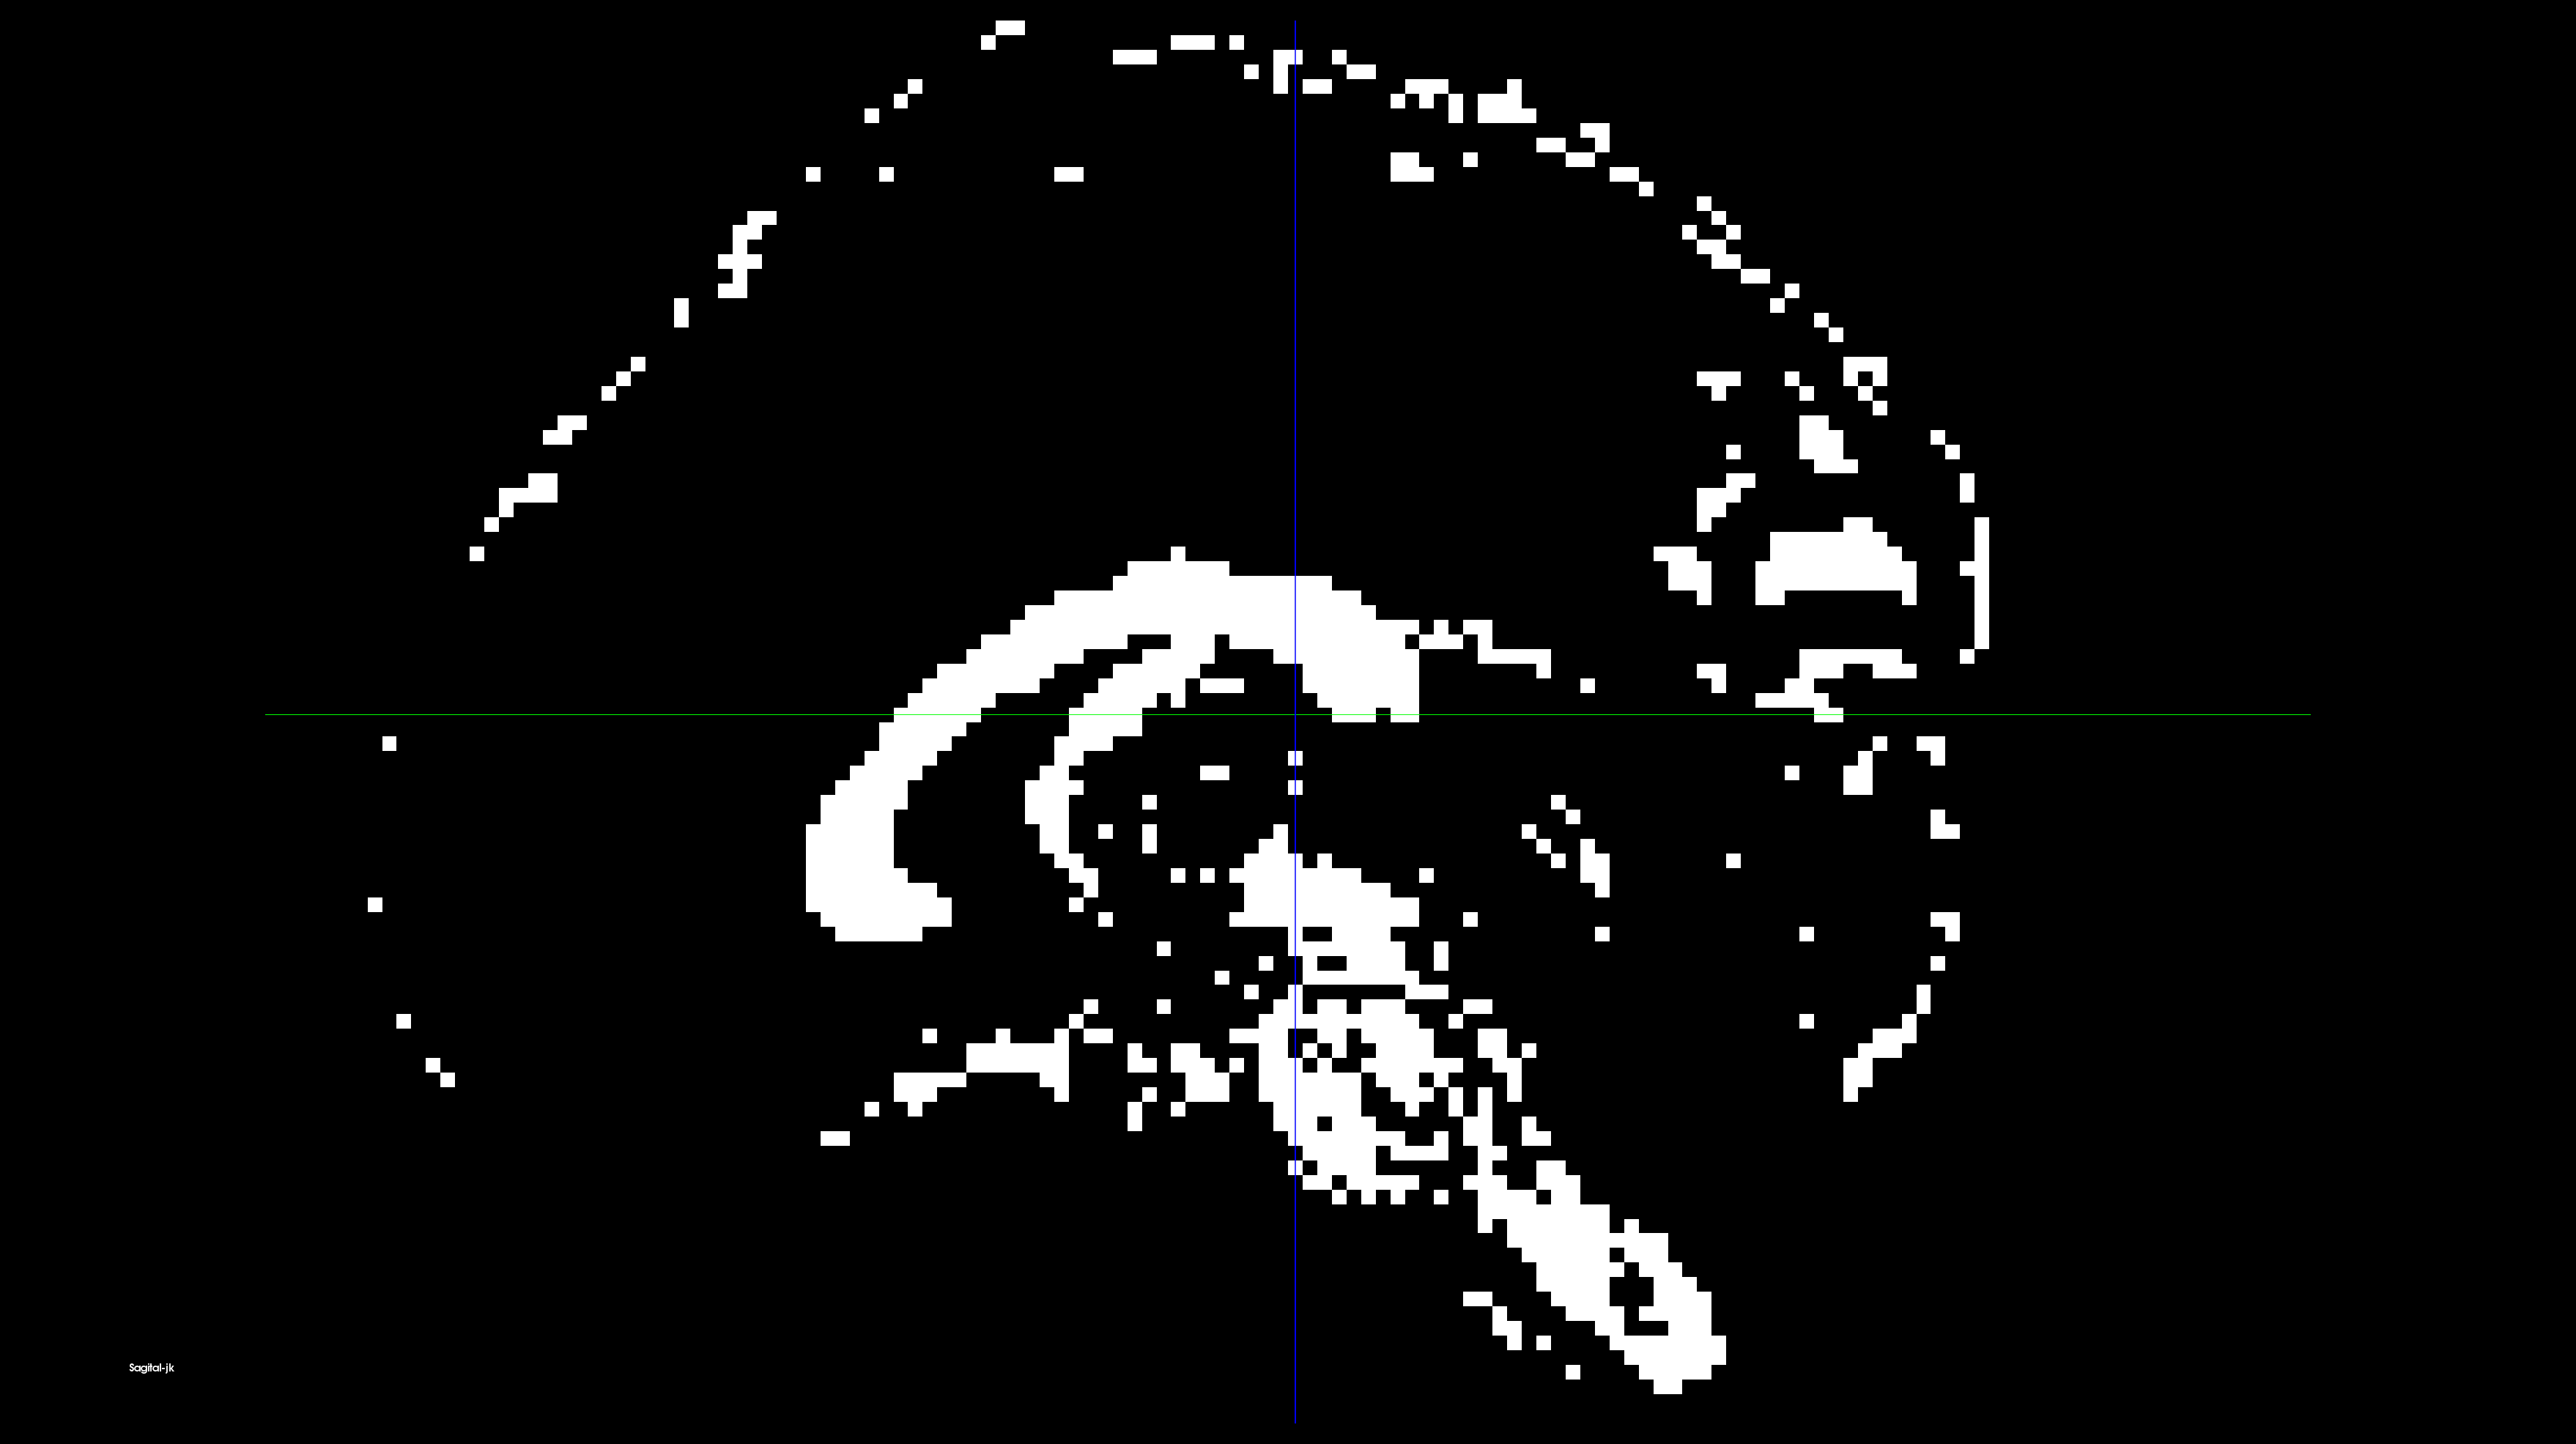
\includegraphics[width=1\linewidth]{imgs/fa_02threshold.png}
        \caption{Sagital cut at (70, 70, 48) for a FA threshold of 0.2.}
        \label{fig:fa_threshold}
      \end{figure}

      This region has the following statistics:

      \begin{tabular}{| c | c | c |}
        \hline
        Number of voxels & FA mean & FA Standard Deviation \\ \hline
        166316 & 0.3854053 & 0.1307380 \\ \hline
      \end{tabular}

      .\newline

      Finally, I first tried to run it with perfect anisotropy and isotropy parameters with no relaxation which produced empty masks for both cases as expected.

      \newpage

      \subsubsection{Relaxed perfect anisotropy and isotropy}
      Then following I've ran the eigenvalues threshold with relaxations first for the perfect anisotropy case producing the following chart:

      \begin{figure}[H]
        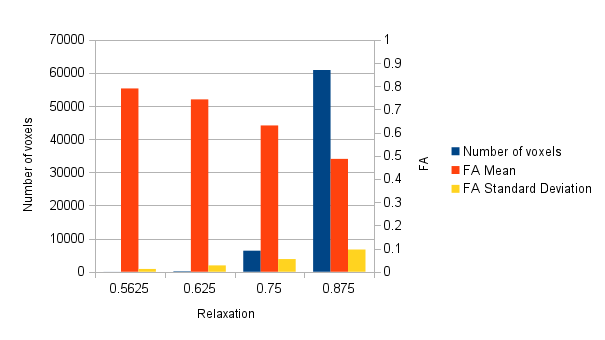
\includegraphics[width=1\linewidth]{imgs/perfect_anisotropy_relaxed_chart.png}
        \caption{Evolution of the statistics accordingly to the relaxation increase.}
        \label{fig:perf-ani-chart}
      \end{figure}

      The first three steps gave really small regions. But for the fourth the region size increased significantly with some loss on the FA mean value:

      \begin{figure}[H]
        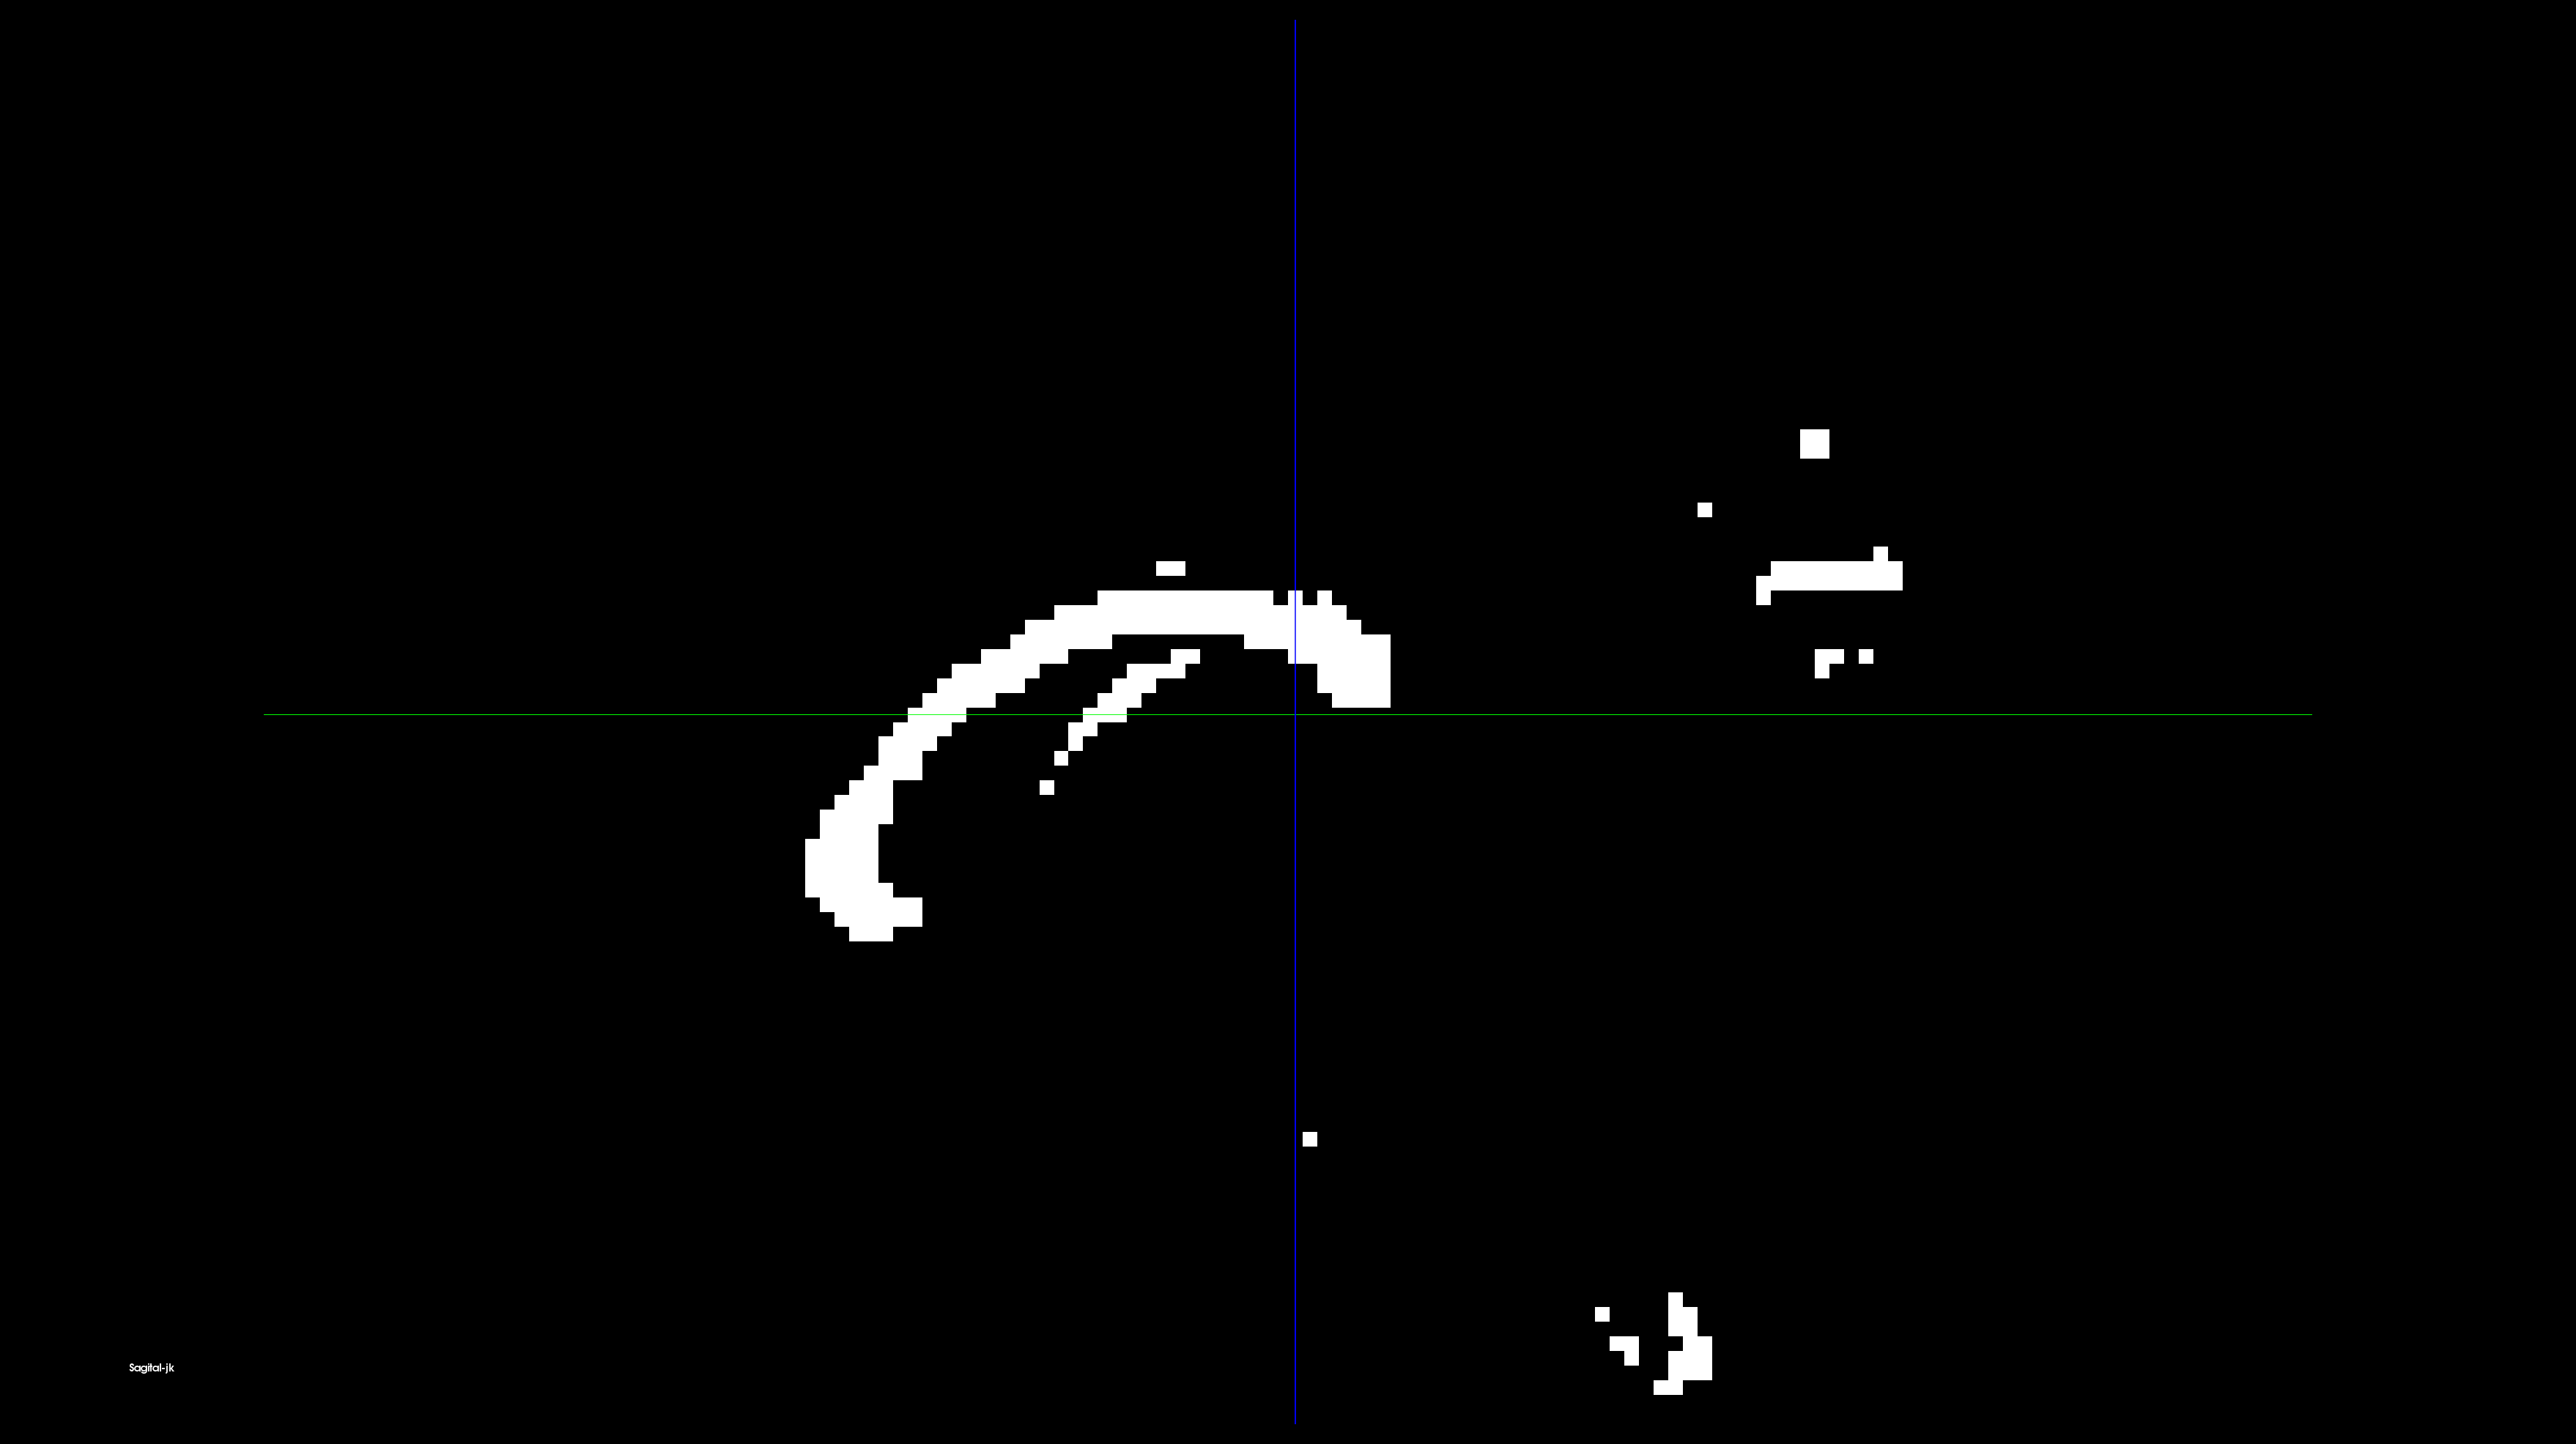
\includegraphics[width=1\linewidth]{imgs/eg_10_10_00_0875.png}
        \caption{Sagital cut at (70, 70, 48) for a perfect anisotropy threshold relaxed to 0.875.}
        \label{fig:perf-ani-0875}
      \end{figure}

      Which looks like like a subset of the FA threshold (\ref{fig:fa_threshold}).

      Next I've repeated the experiment relaxing the threshold for the perfect isotropy case, producing the following statistics:

      \begin{figure}[H]
        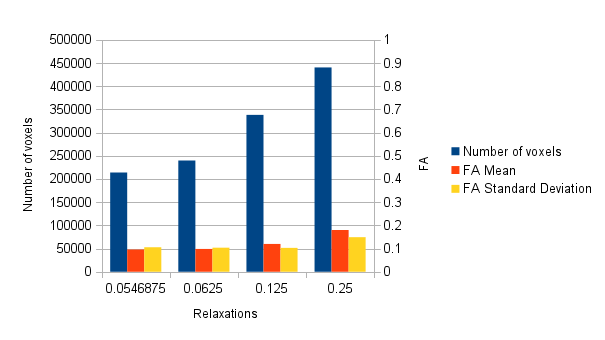
\includegraphics[width=1\linewidth]{imgs/perfect_isotropy_relaxed_chart.png}
        \caption{Evolution of the statistics accordingly to the relaxation increase.}
        \label{fig:perf-ani-chart}
      \end{figure}

      Which we can see the results for each step here:

      \begin{figure}[H]
        \centering

        \begin{subfigure}[t]{.49\textwidth}
          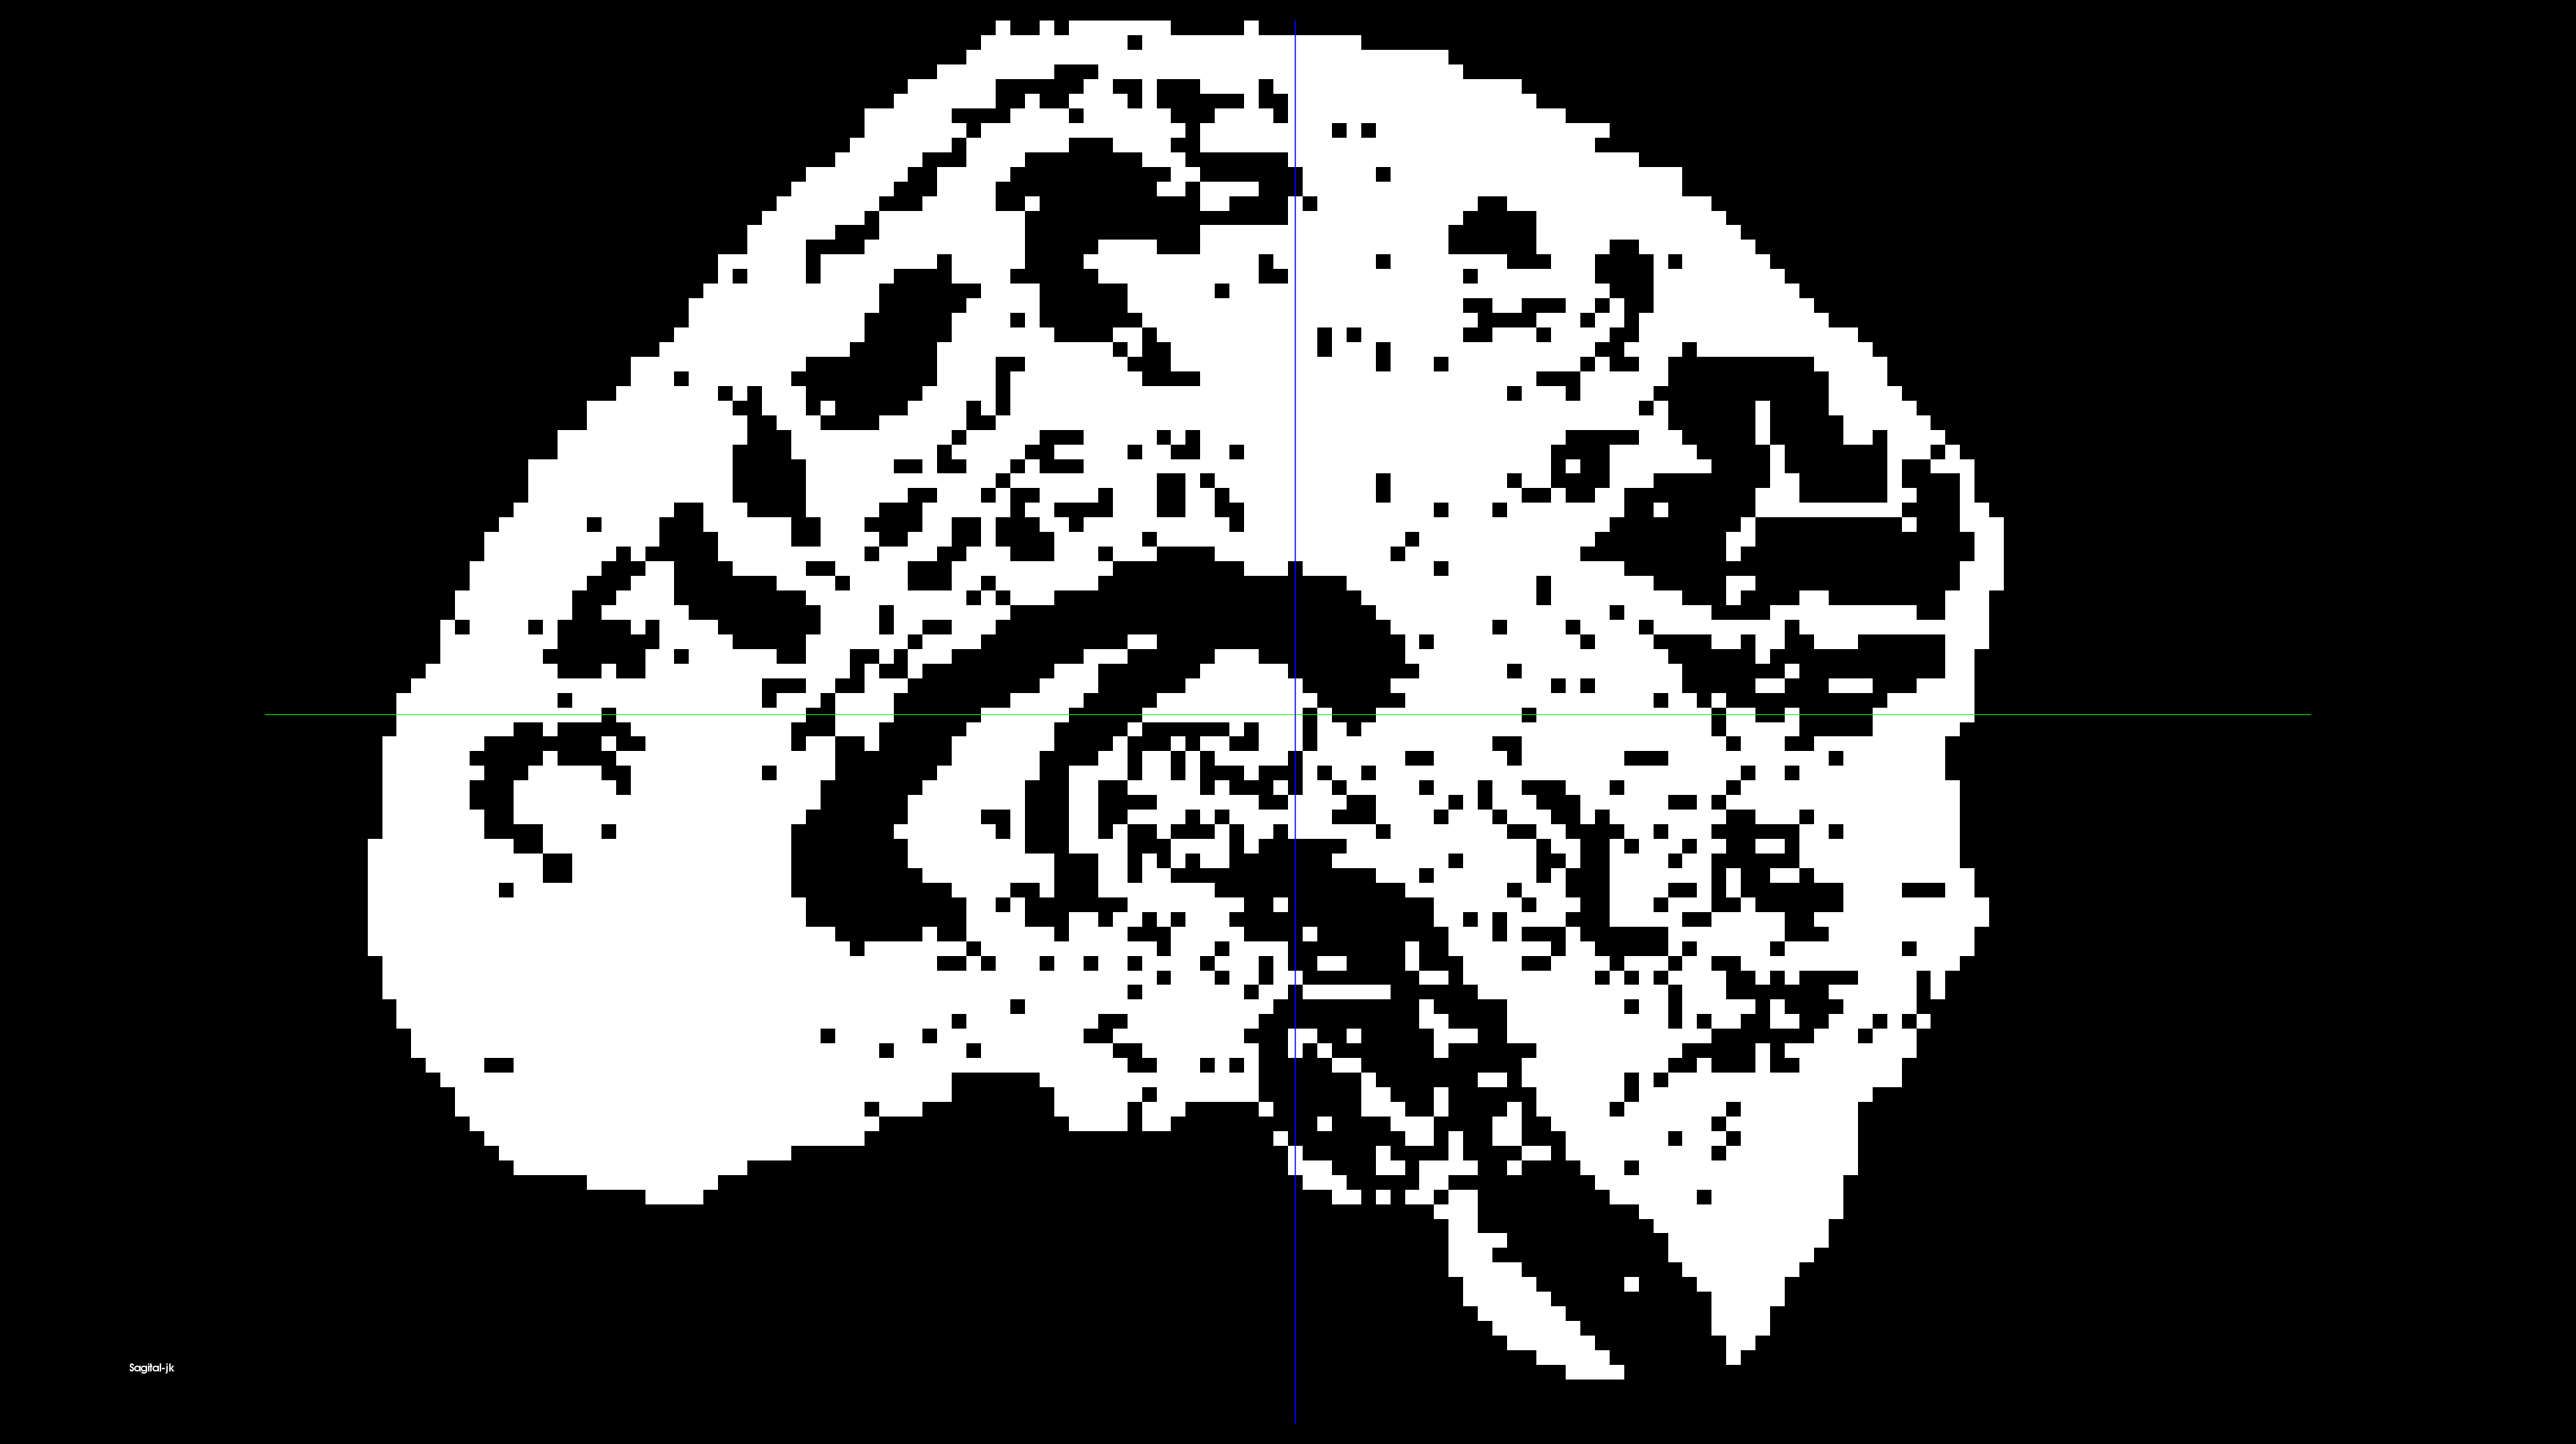
\includegraphics[width=1\linewidth]{imgs/eg_00_00_00_00546875.png}
          \caption{Relaxation at 0.0546875.}
          \label{subfig:perf-iso-0054}
        \end{subfigure}\hfill%
        \begin{subfigure}[t]{.49\textwidth}
          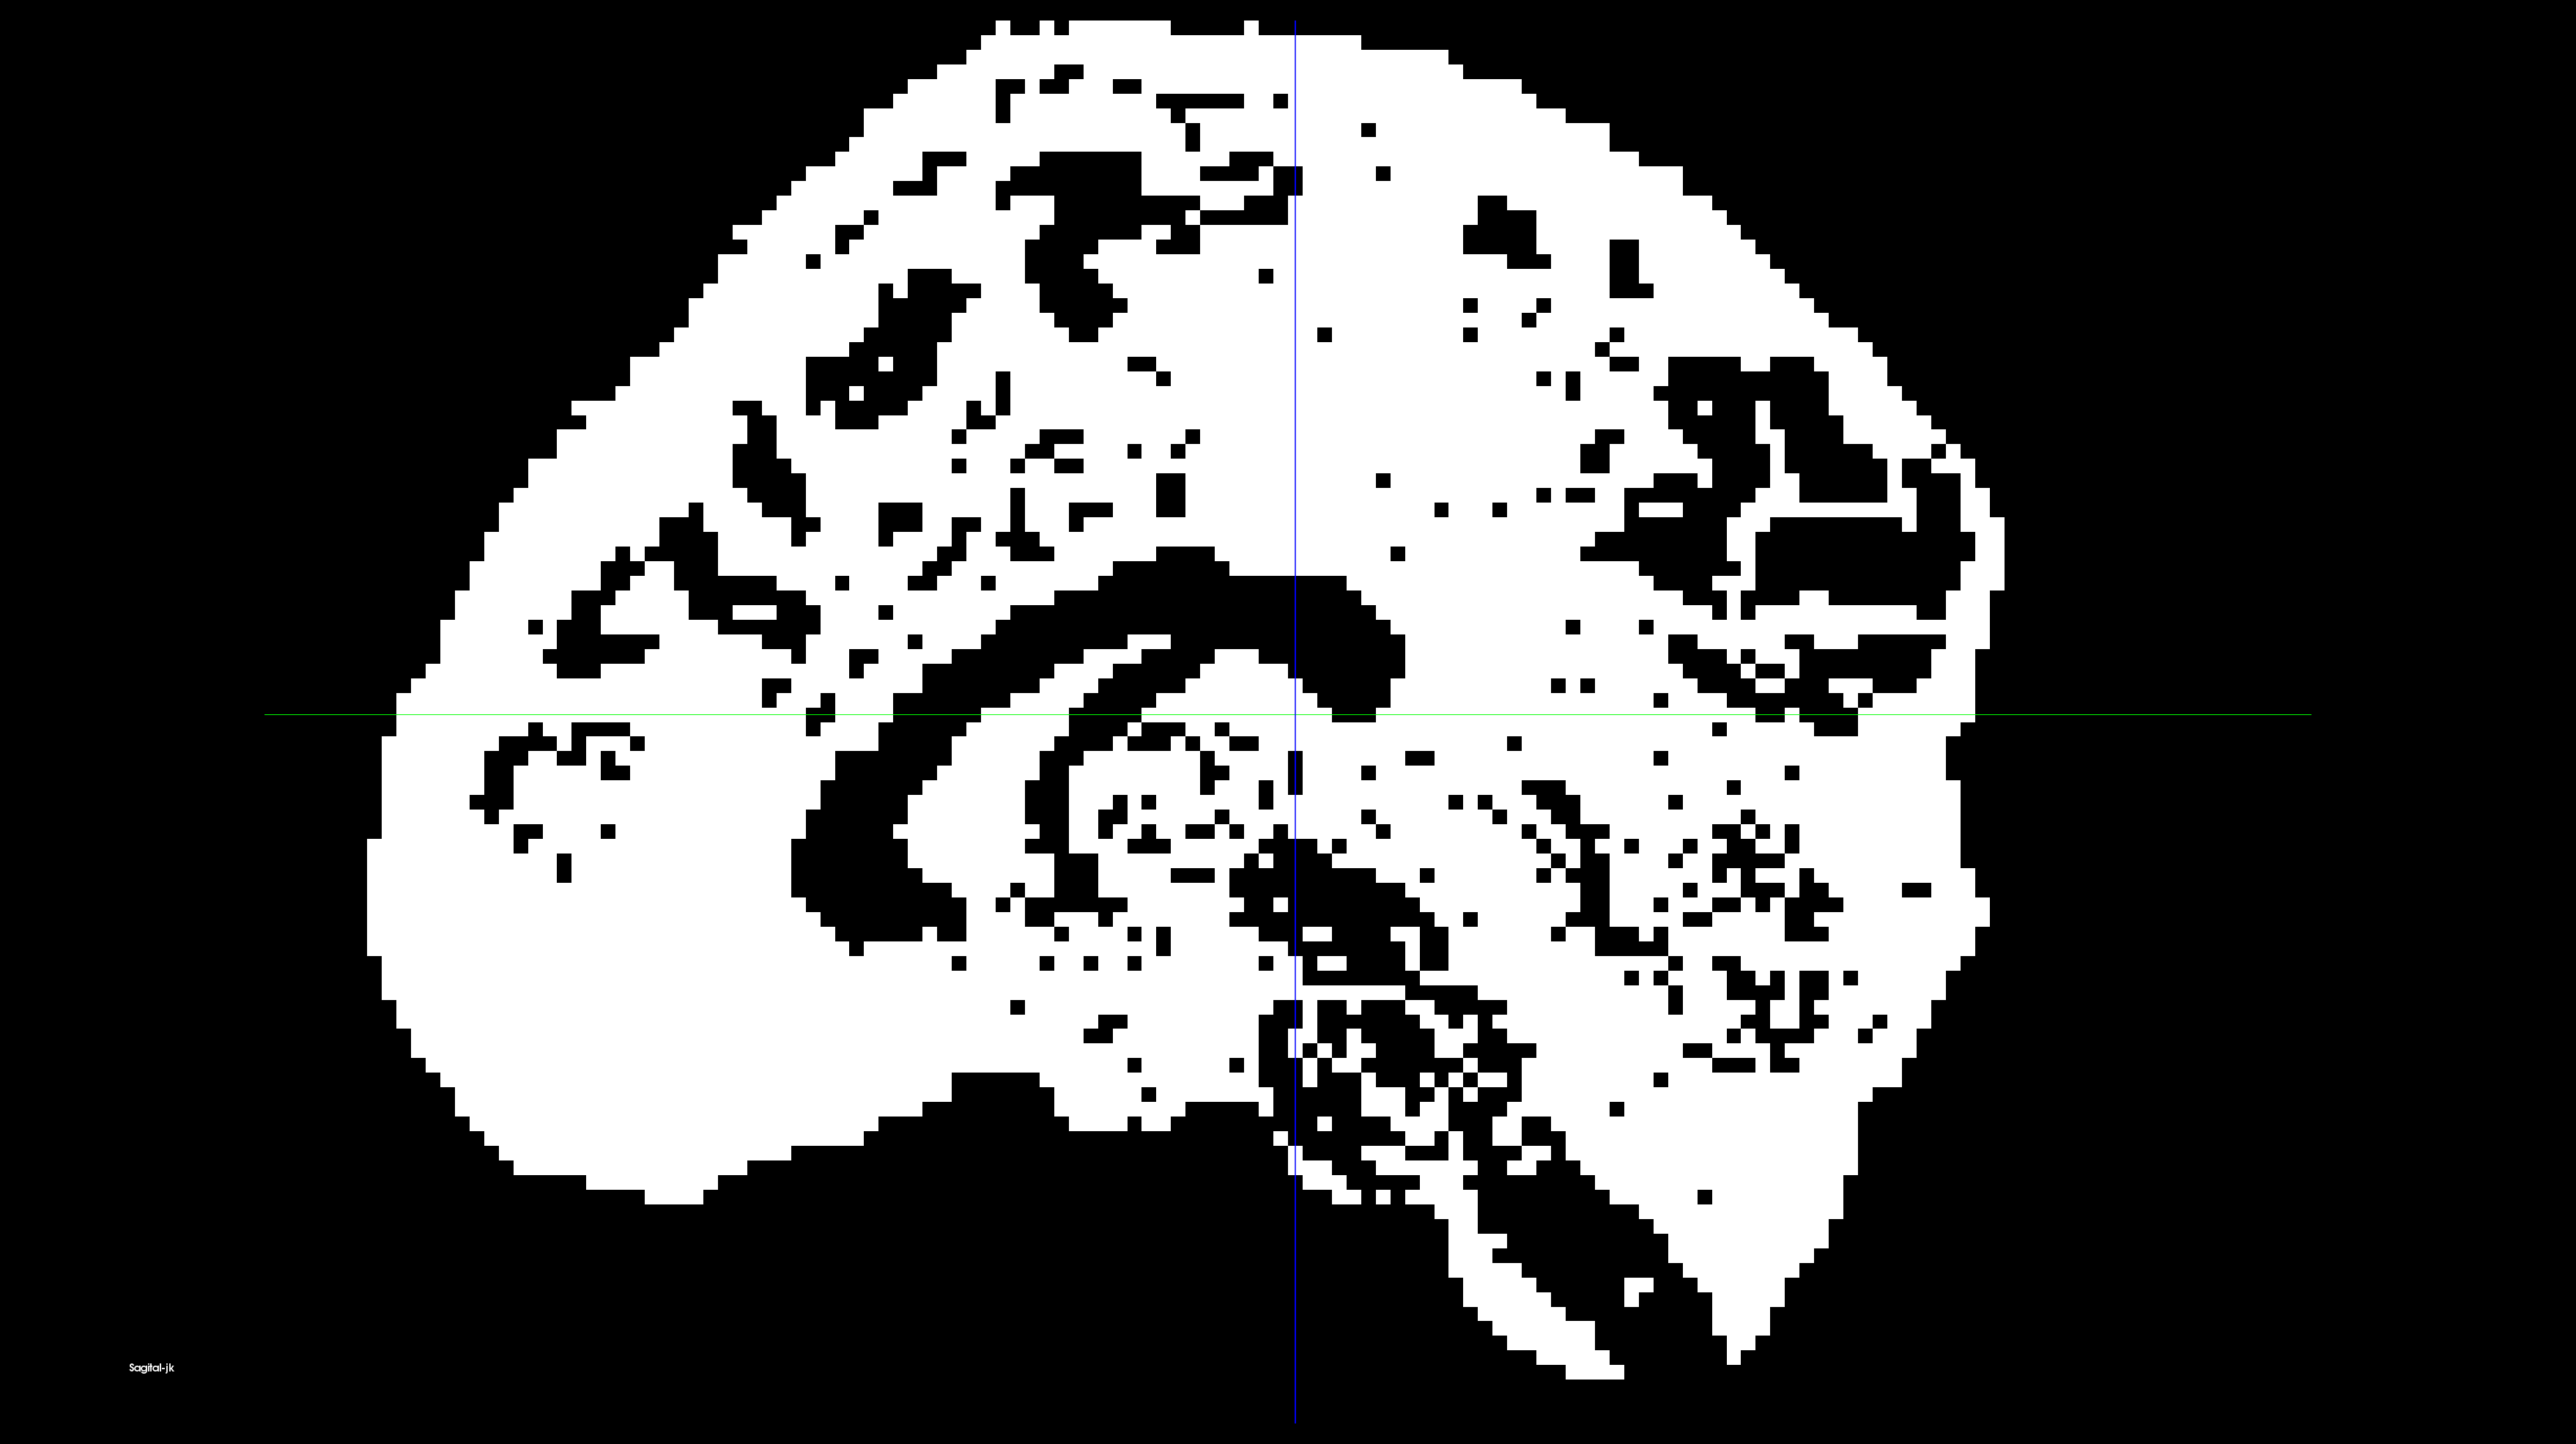
\includegraphics[width=1\linewidth]{imgs/eg_00_00_00_00625.png}
          \caption{Relaxation at 0.0625.}
          \label{subfig:perf-iso-0062}
        \end{subfigure}\hfill\\
        \begin{subfigure}[t]{.49\textwidth}
          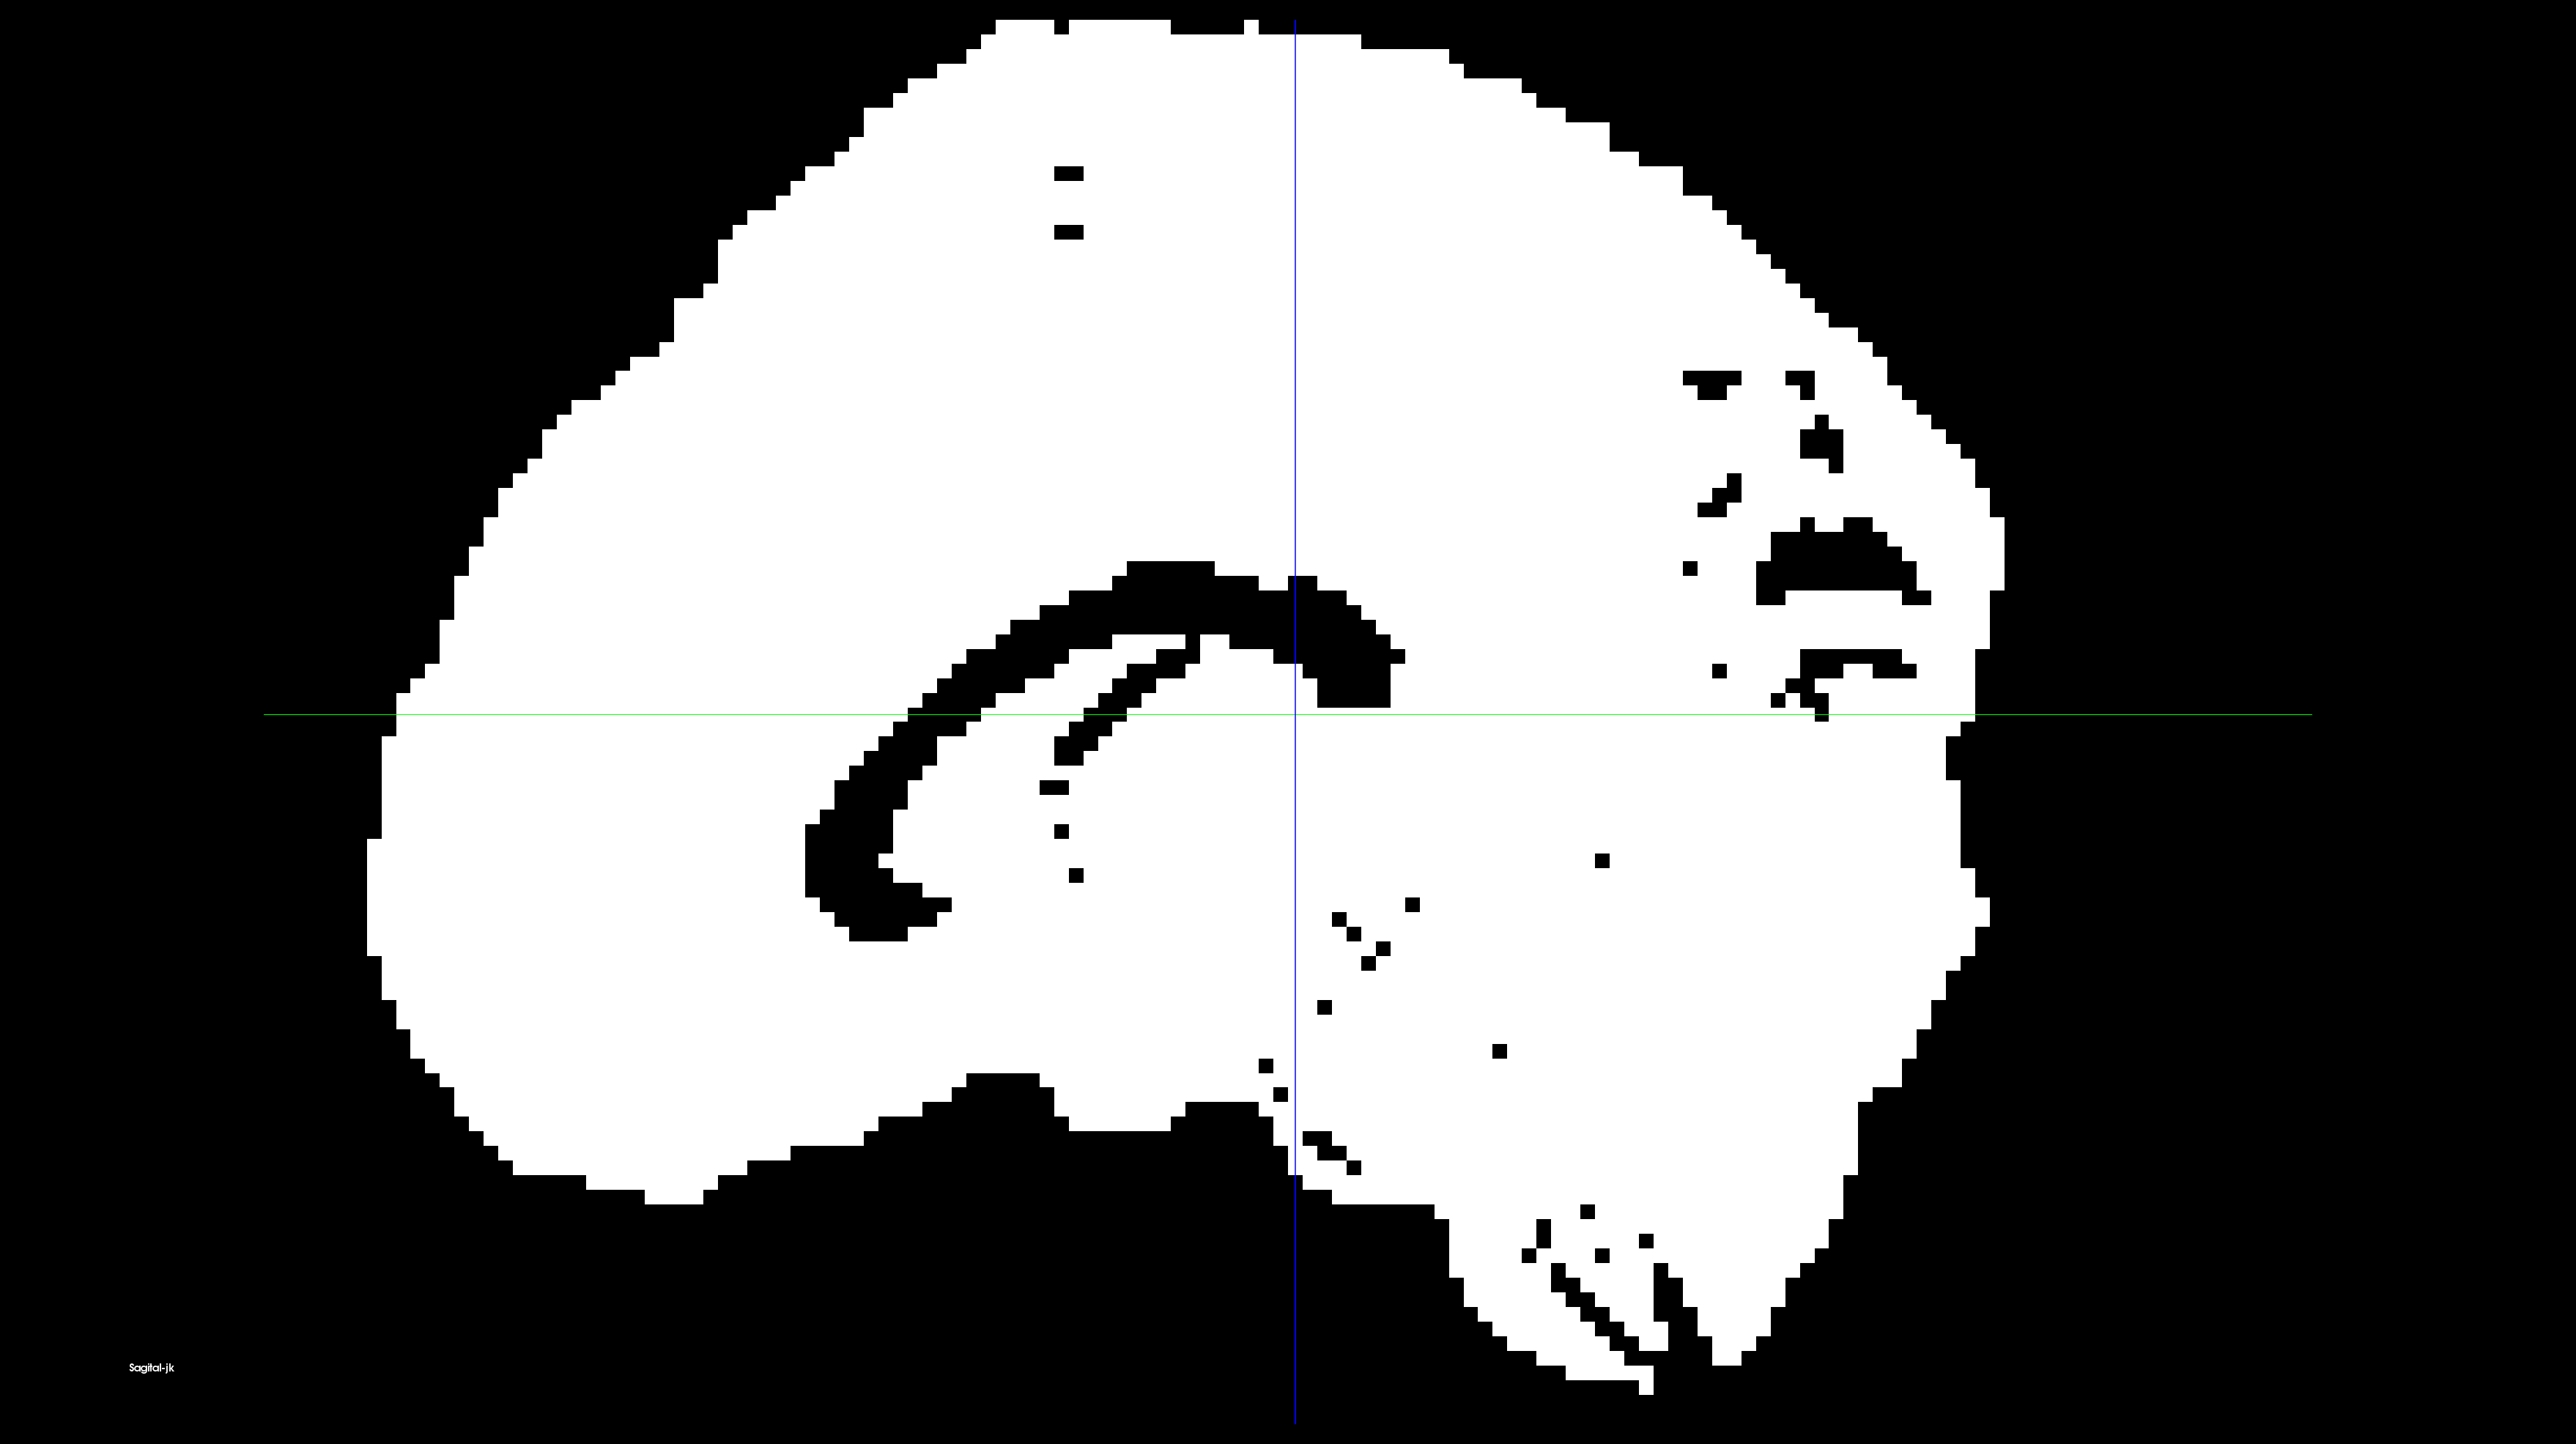
\includegraphics[width=1\linewidth]{imgs/eg_00_00_00_0125.png}
          \caption{Relaxation at 0.125.}
          \label{subfig:perf-iso-0125}
        \end{subfigure}\hfill%
        \begin{subfigure}[t]{.49\textwidth}
          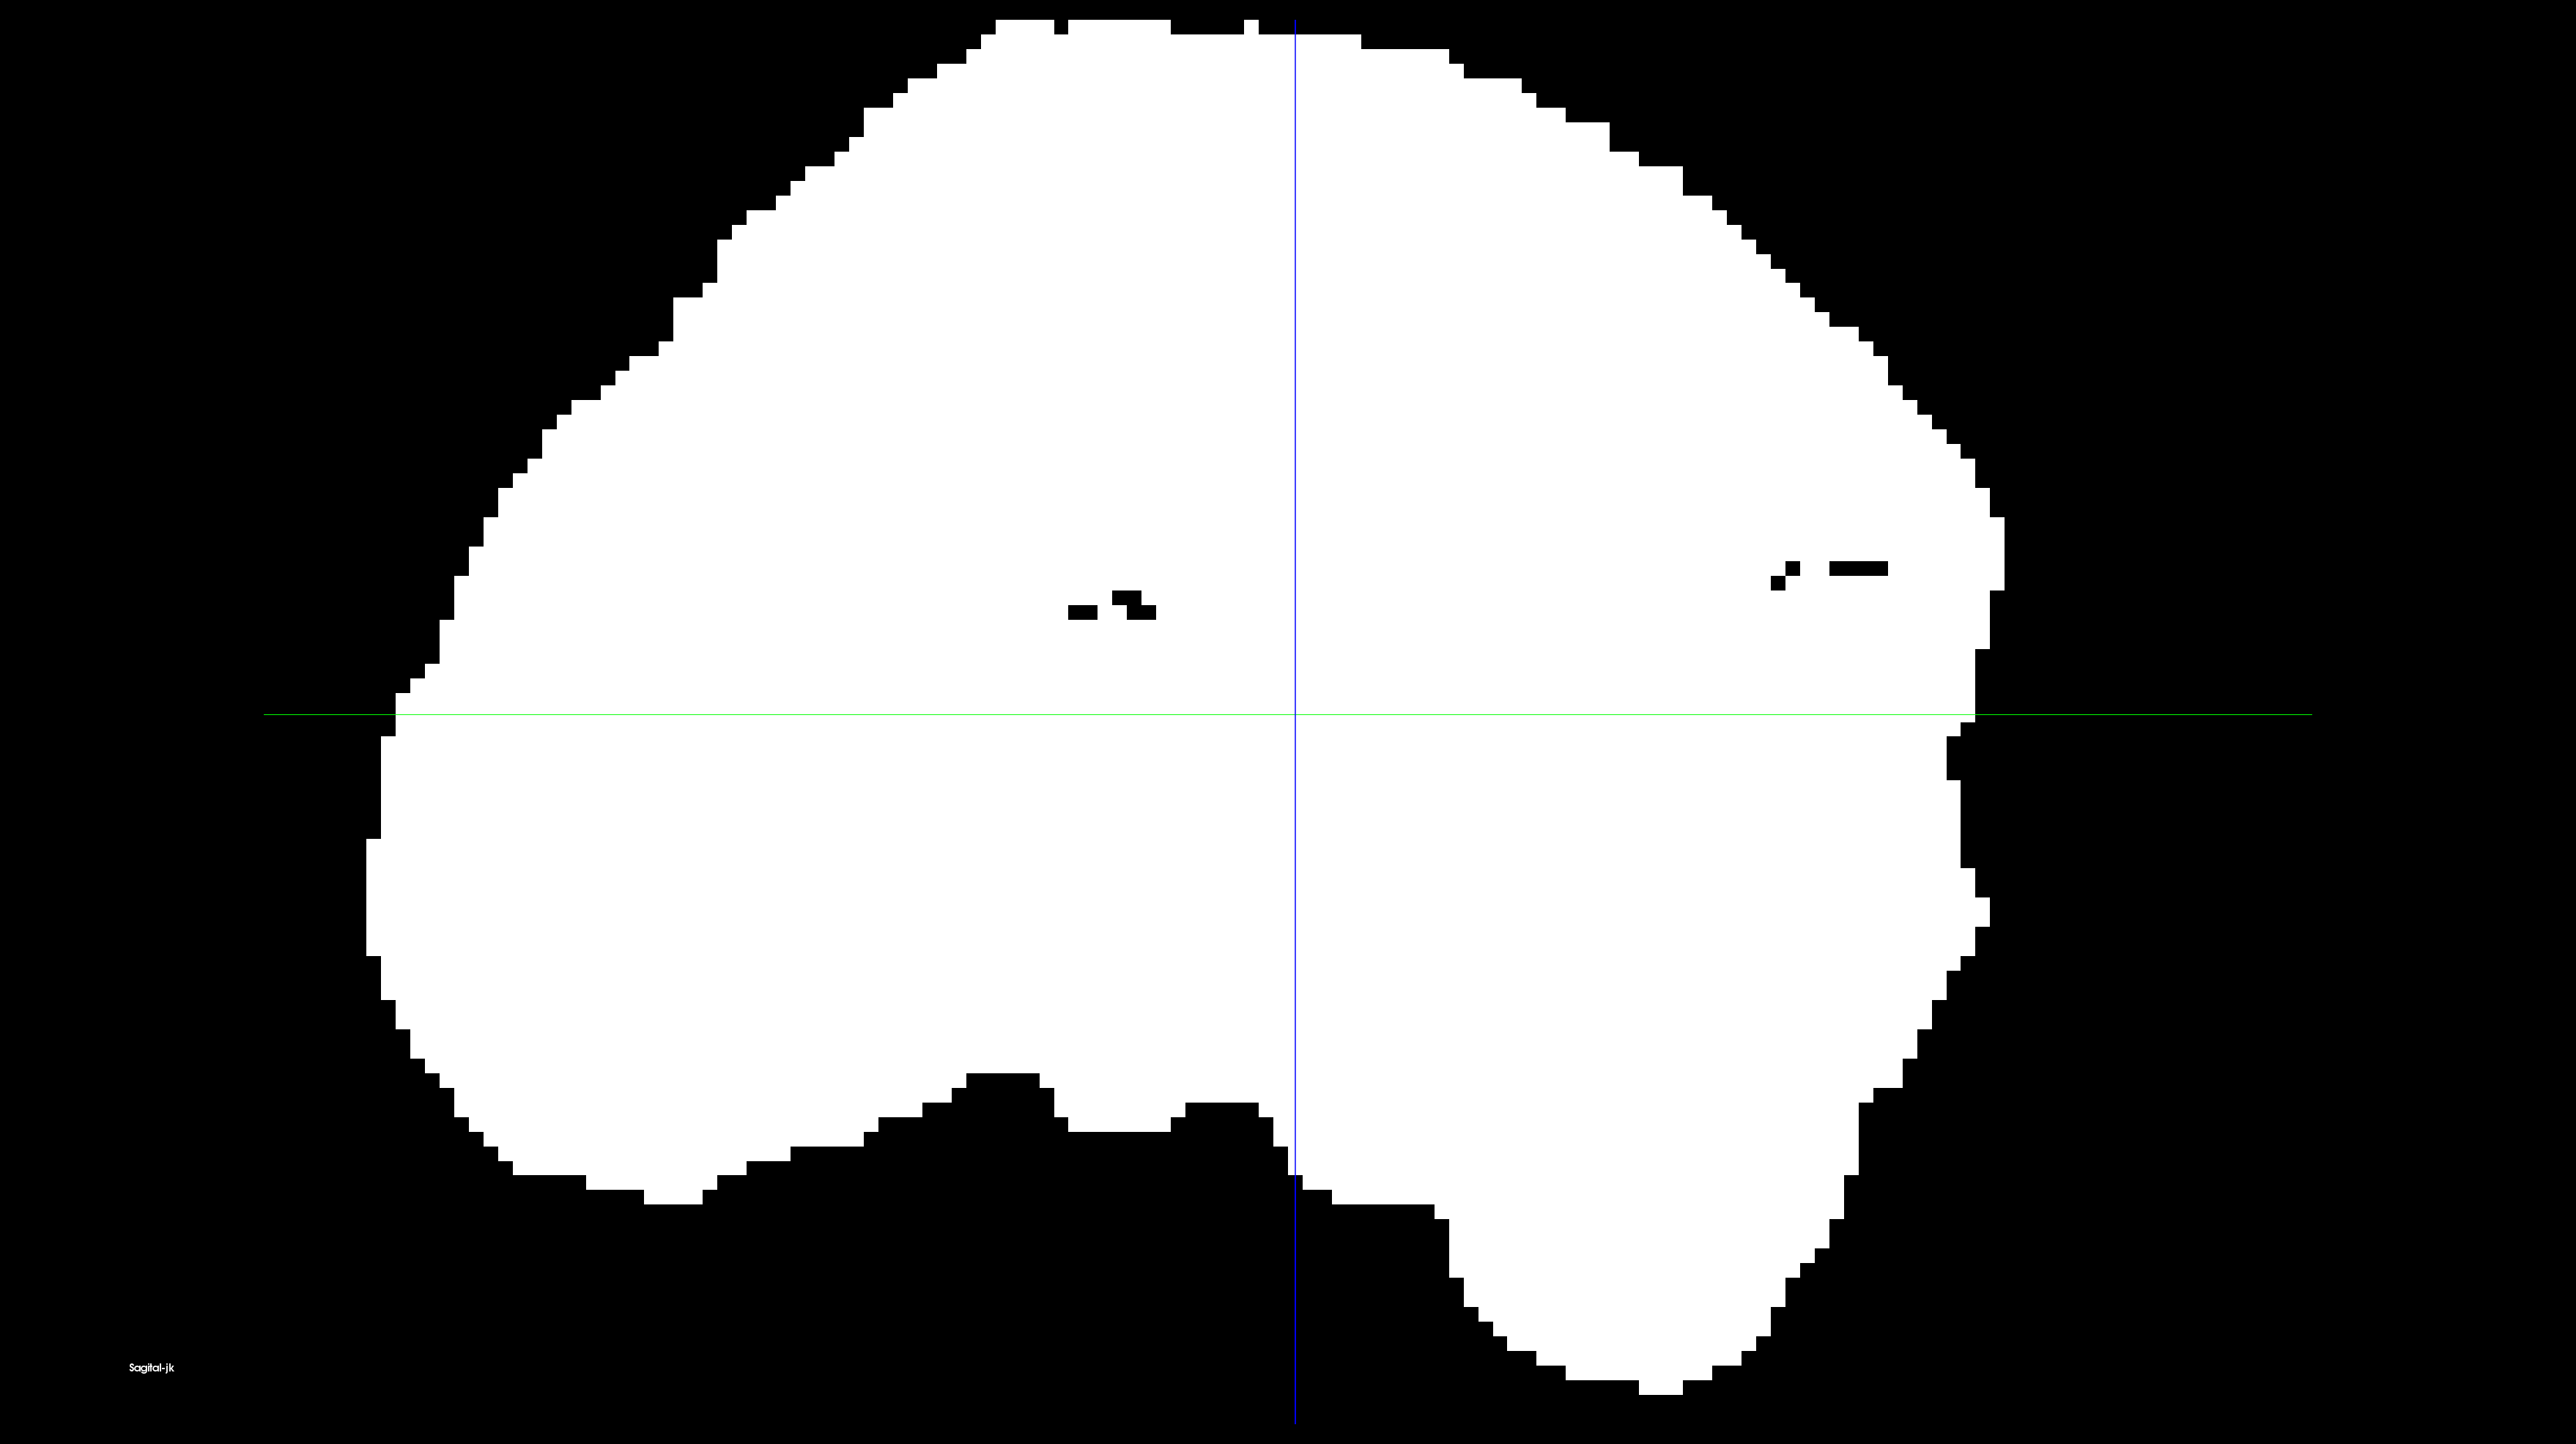
\includegraphics[width=1\linewidth]{imgs/eg_00_00_00_025.png}
          \caption{Relaxation at 0.25.}
          \label{subfig:perf-iso-025}
        \end{subfigure}

        \caption{Sagital cut at (70, 70, 48) for a perfect isotropy steps}
      \end{figure}

  \section{Watersheds}
    Unfortunately, almost none of the watersheds provided any useful information except for the TV values, but not a lot of information.

    \subsection{Fractional anisotropy (FA)}
    \begin{figure}[H]
      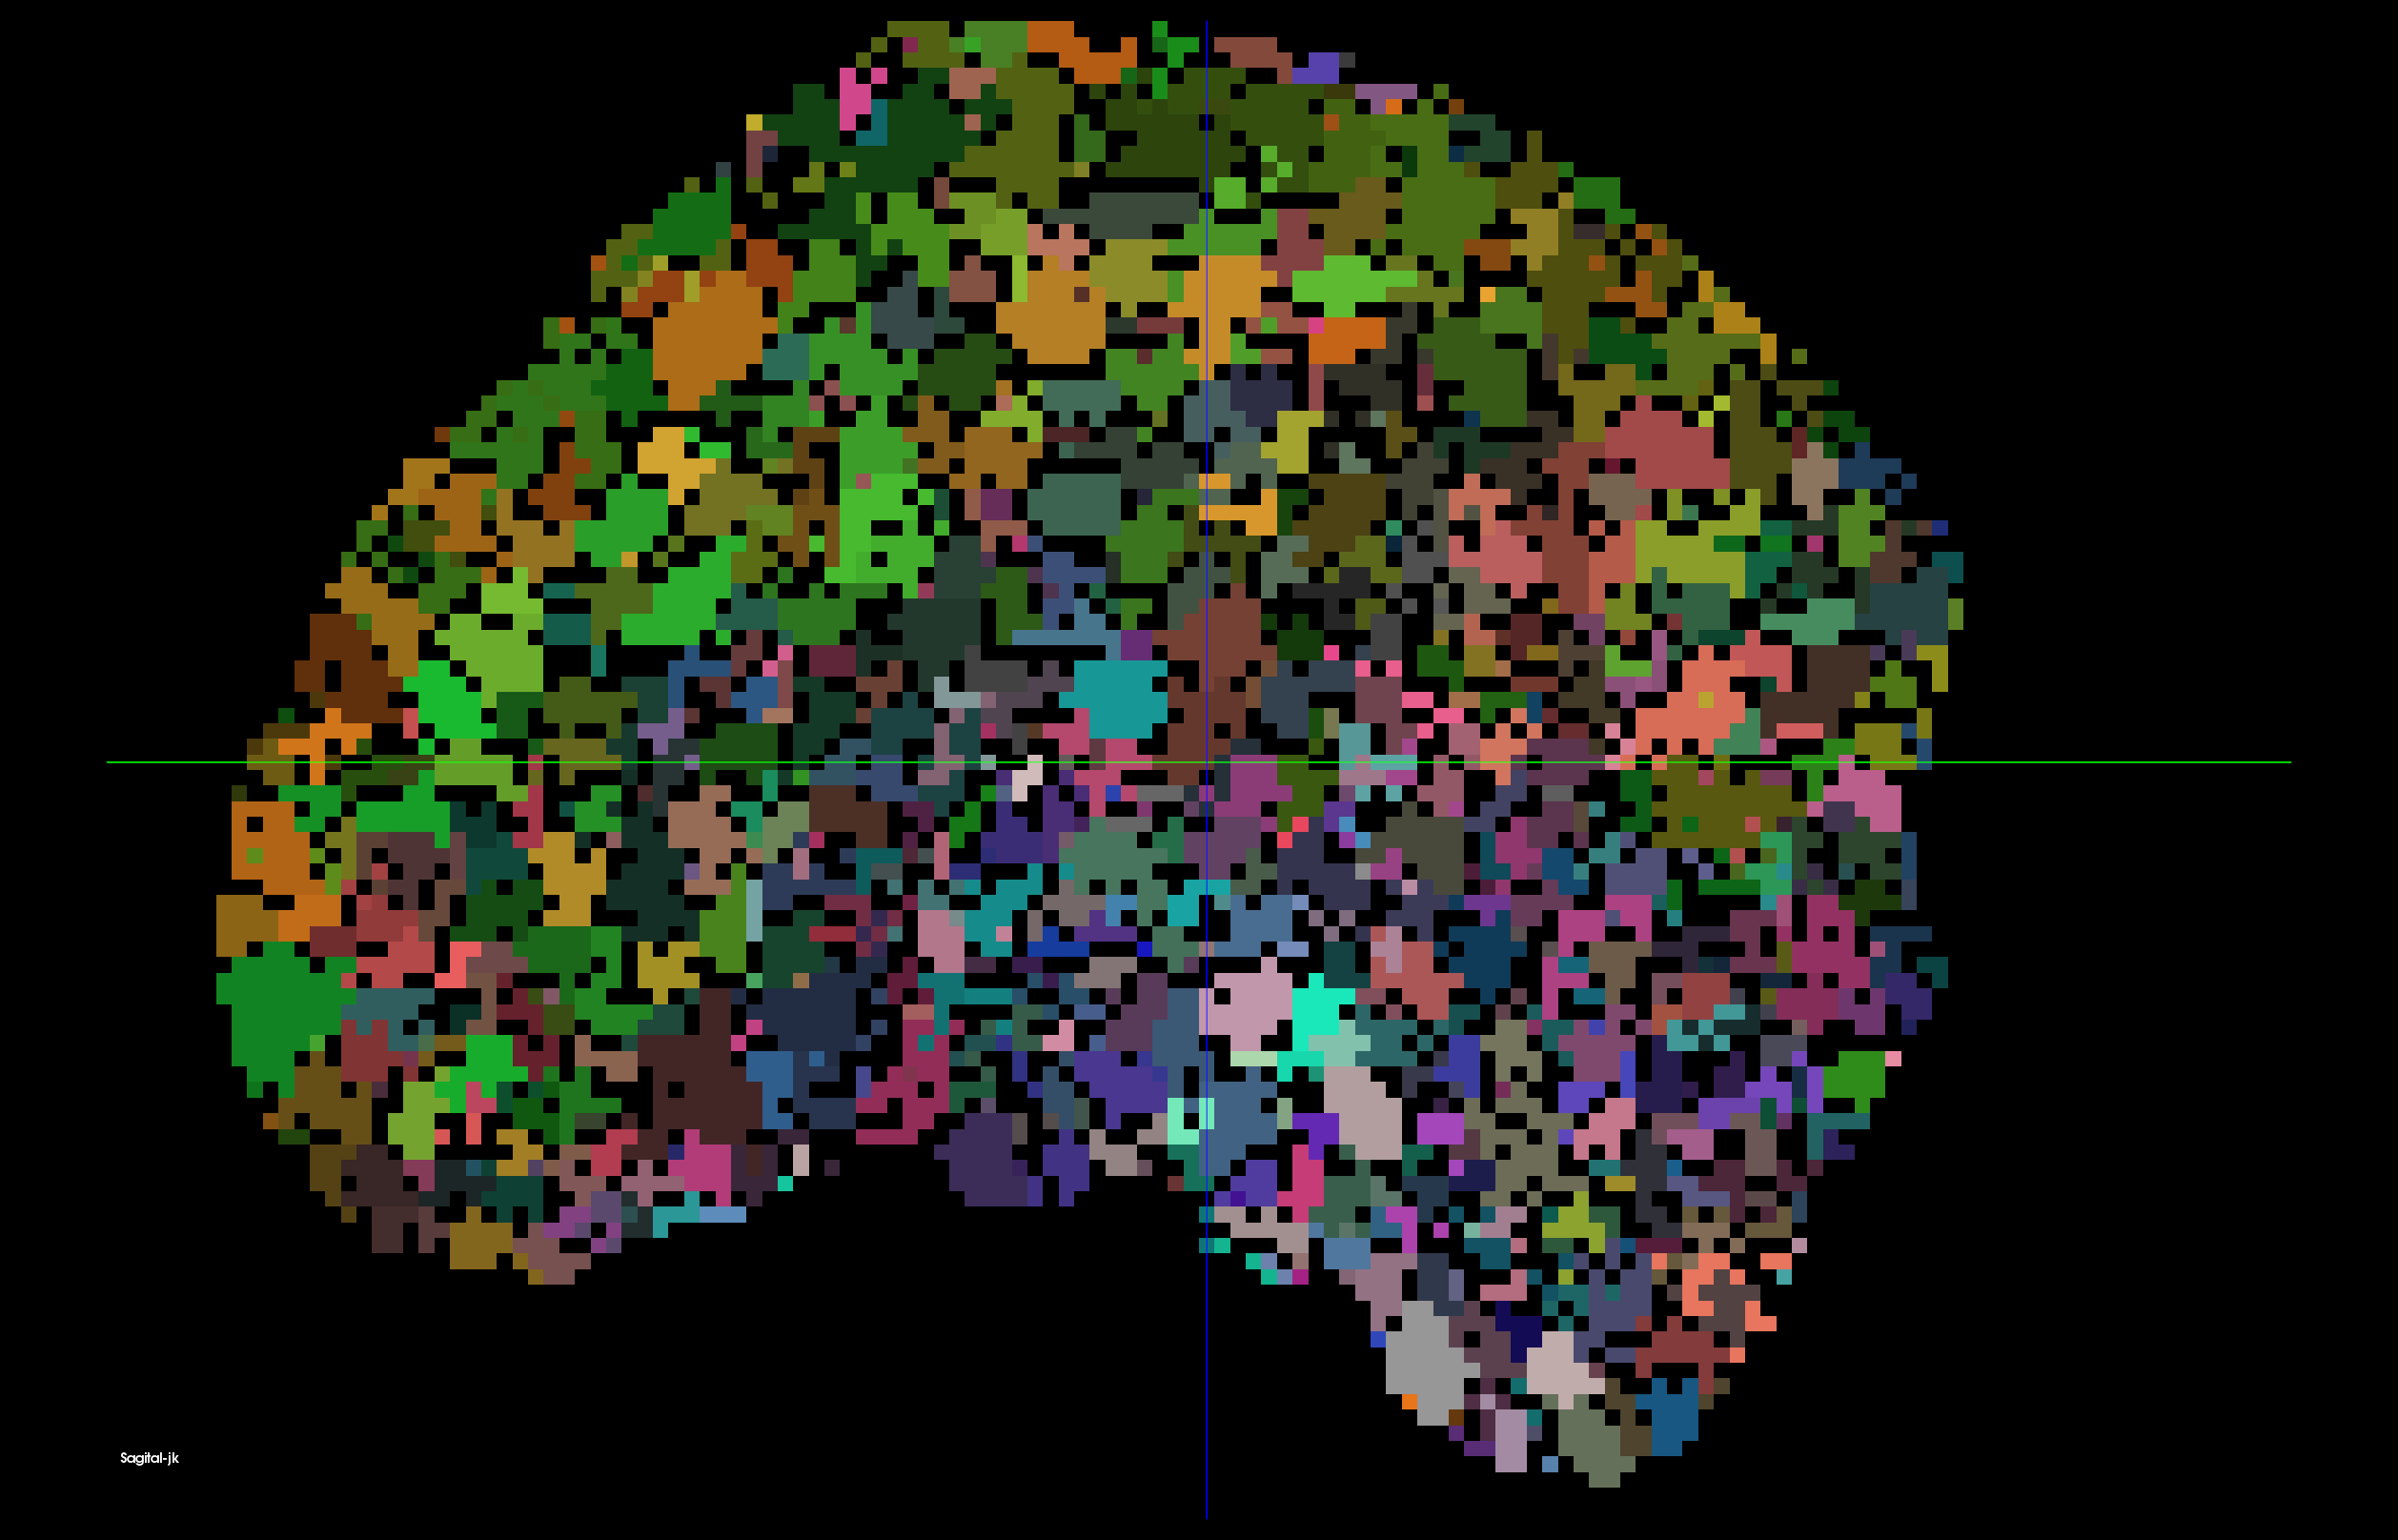
\includegraphics[width=1\linewidth]{imgs/fa_watersheds.png}
      \caption{Sagital cut at (70, 70, 48) for FA watersheds.}
      \label{fig:fa_watersheds}
    \end{figure}

    \subsection{Mean diffusivity (MD)}
    \begin{figure}[H]
      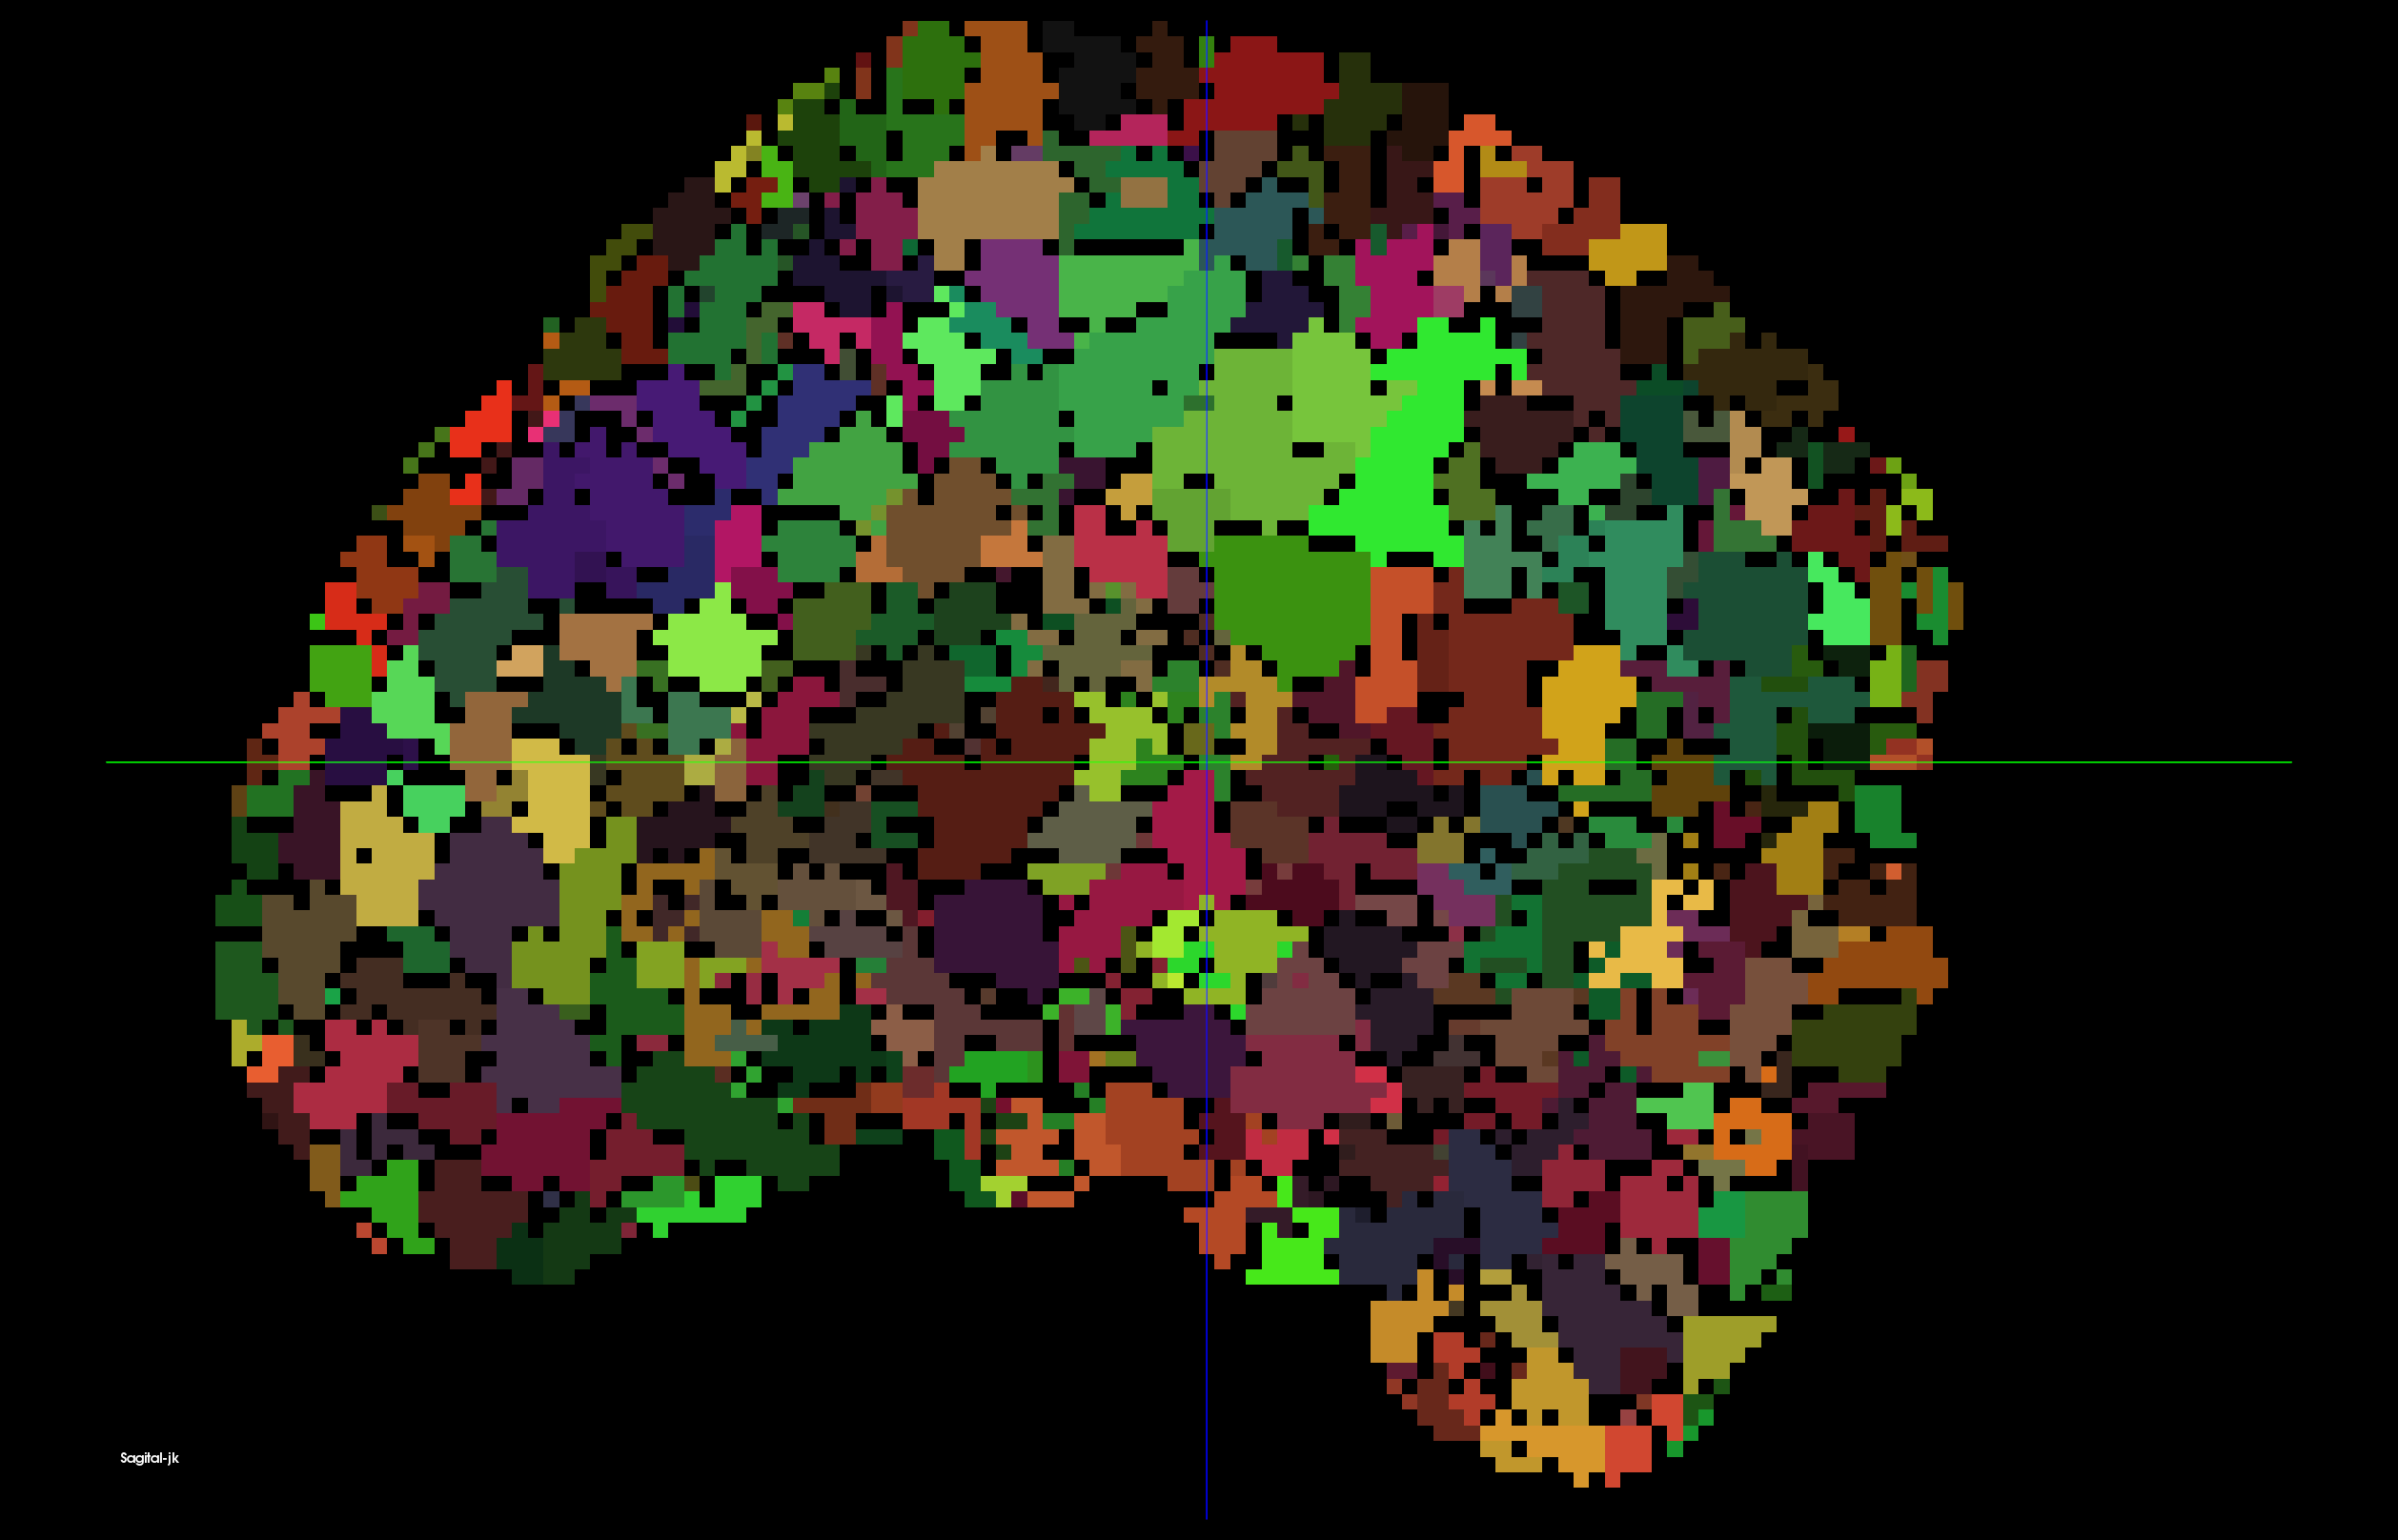
\includegraphics[width=1\linewidth]{imgs/md_watersheds.png}
      \caption{Sagital cut at (70, 70, 48) for MD watersheds.}
      \label{fig:md_watersheds}
    \end{figure}

    \subsection{Radial diffusivity (RD)}
    \begin{figure}[H]
      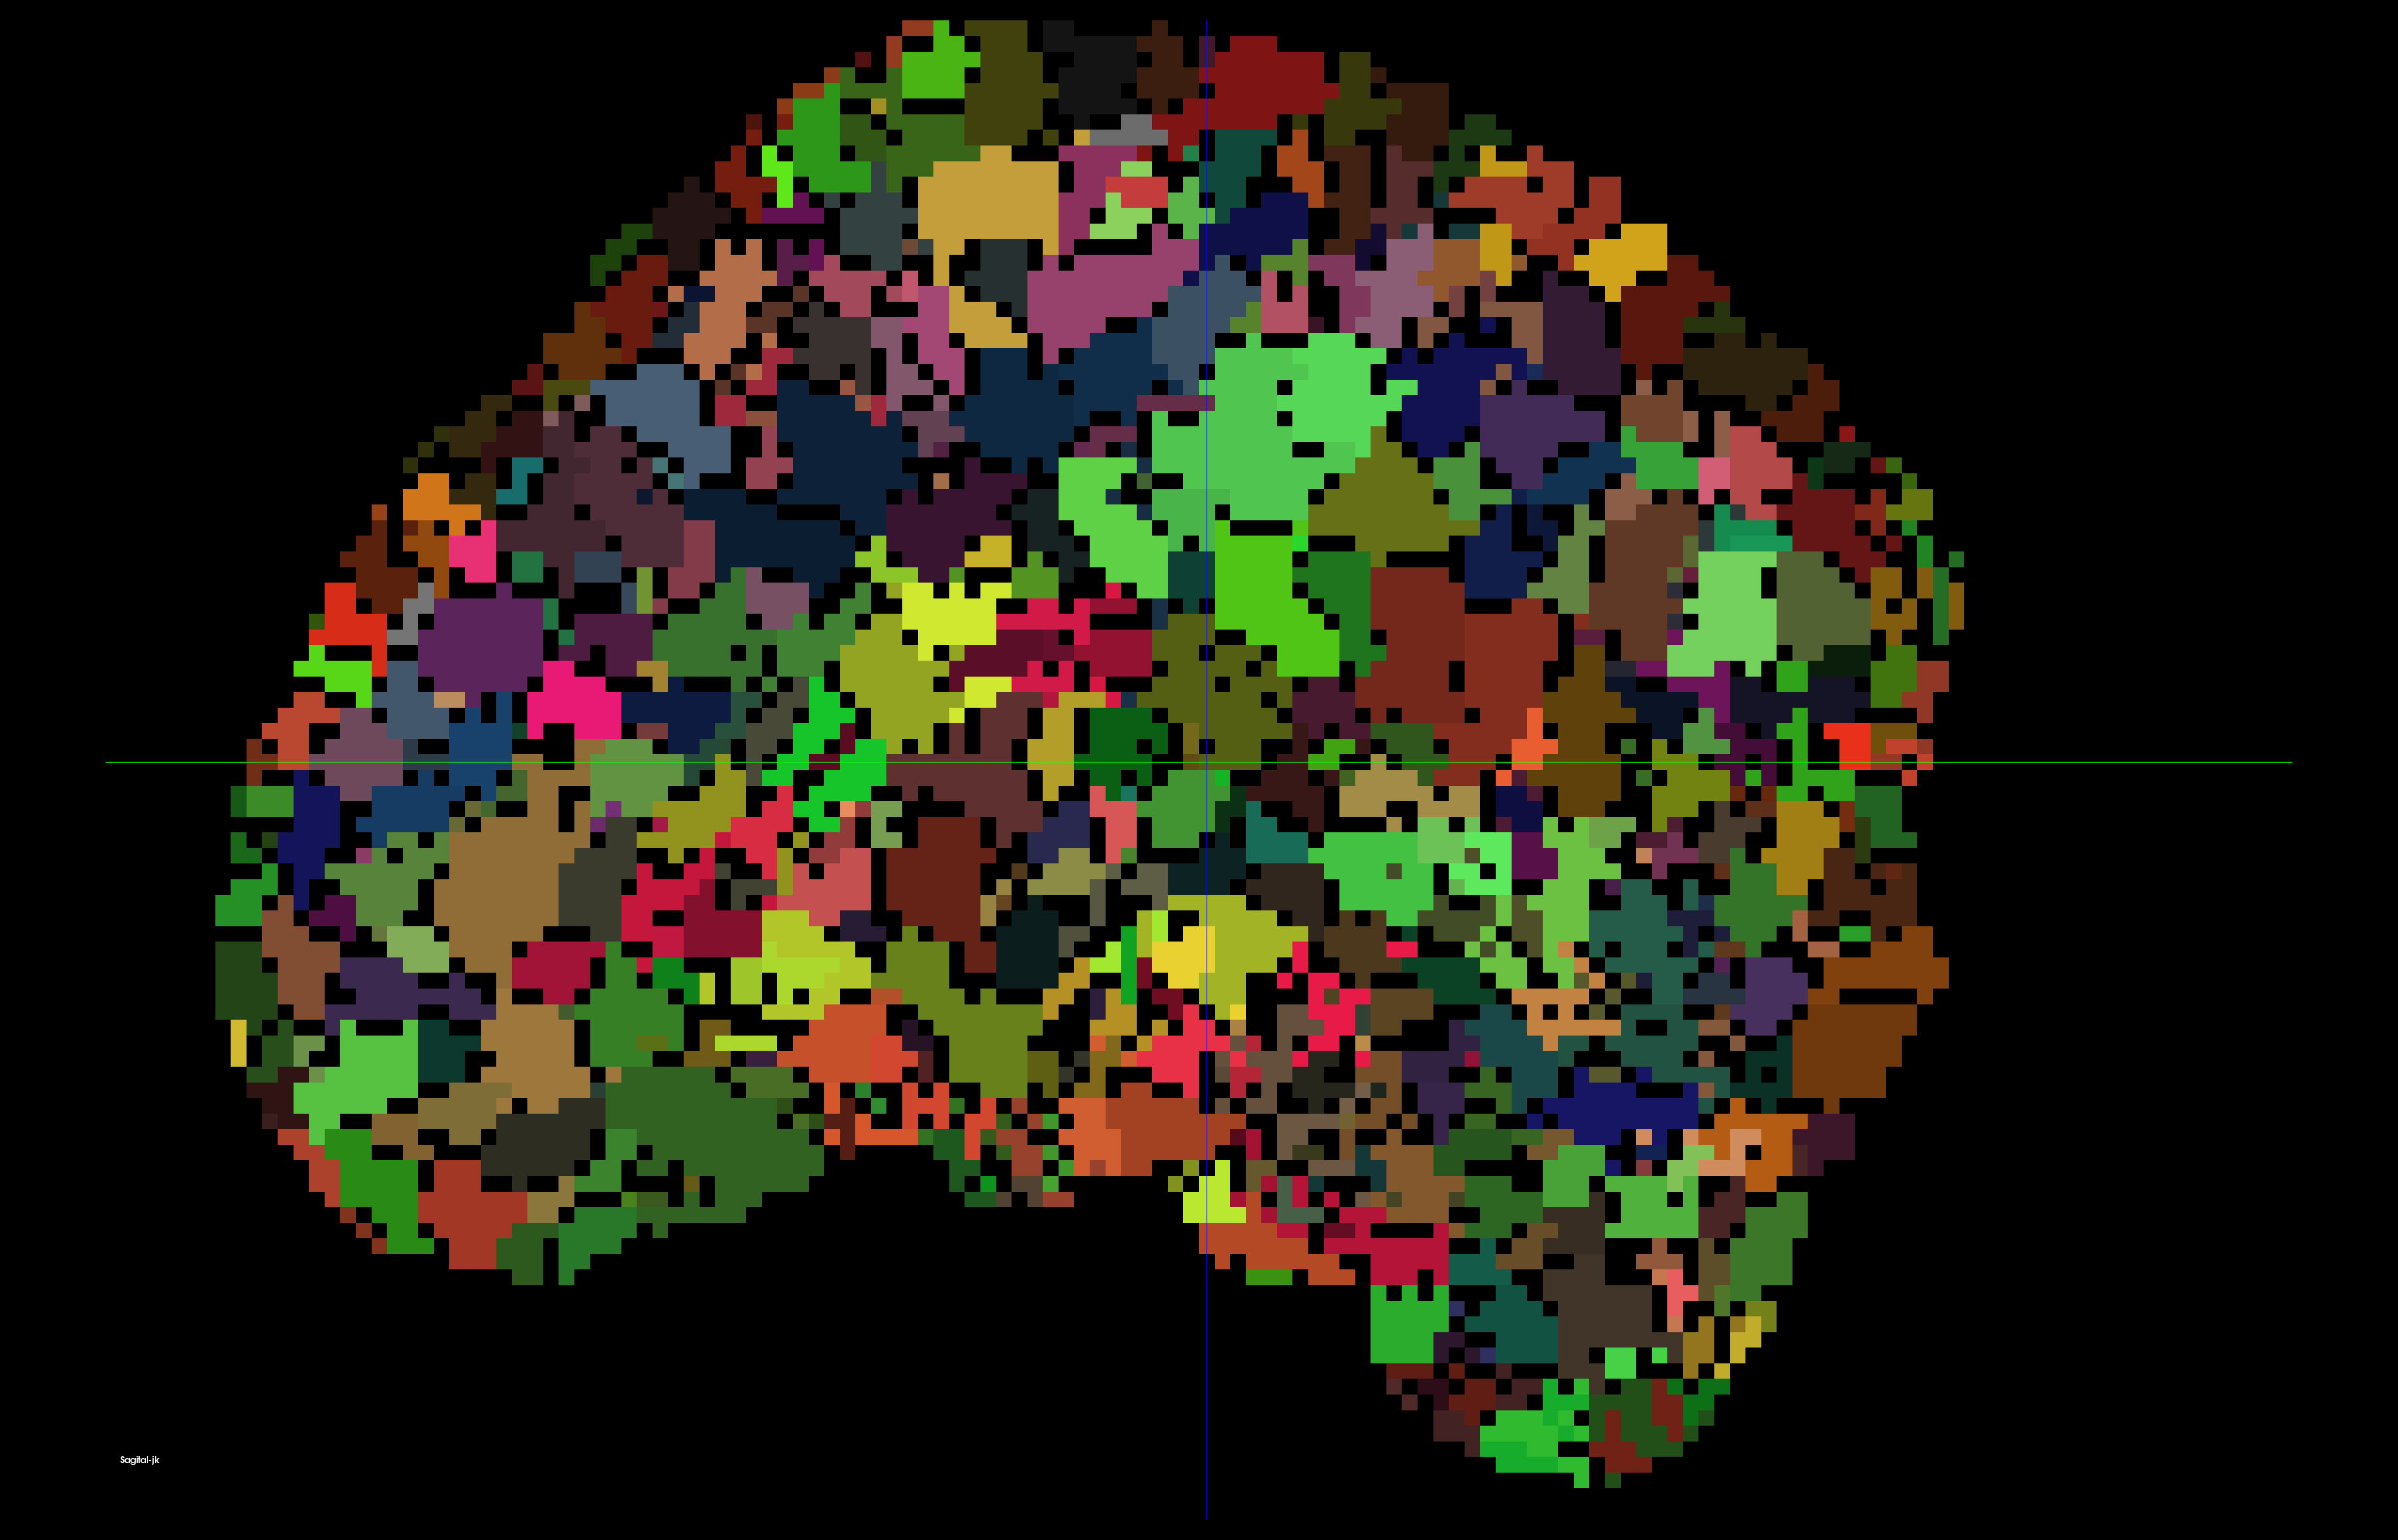
\includegraphics[width=1\linewidth]{imgs/rd_watersheds.png}
      \caption{Sagital cut at (70, 70, 48) for RD watersheds.}
      \label{fig:rd_watersheds}
    \end{figure}

    \subsection{Toroidal Volume (TV)}
    \begin{figure}[H]
      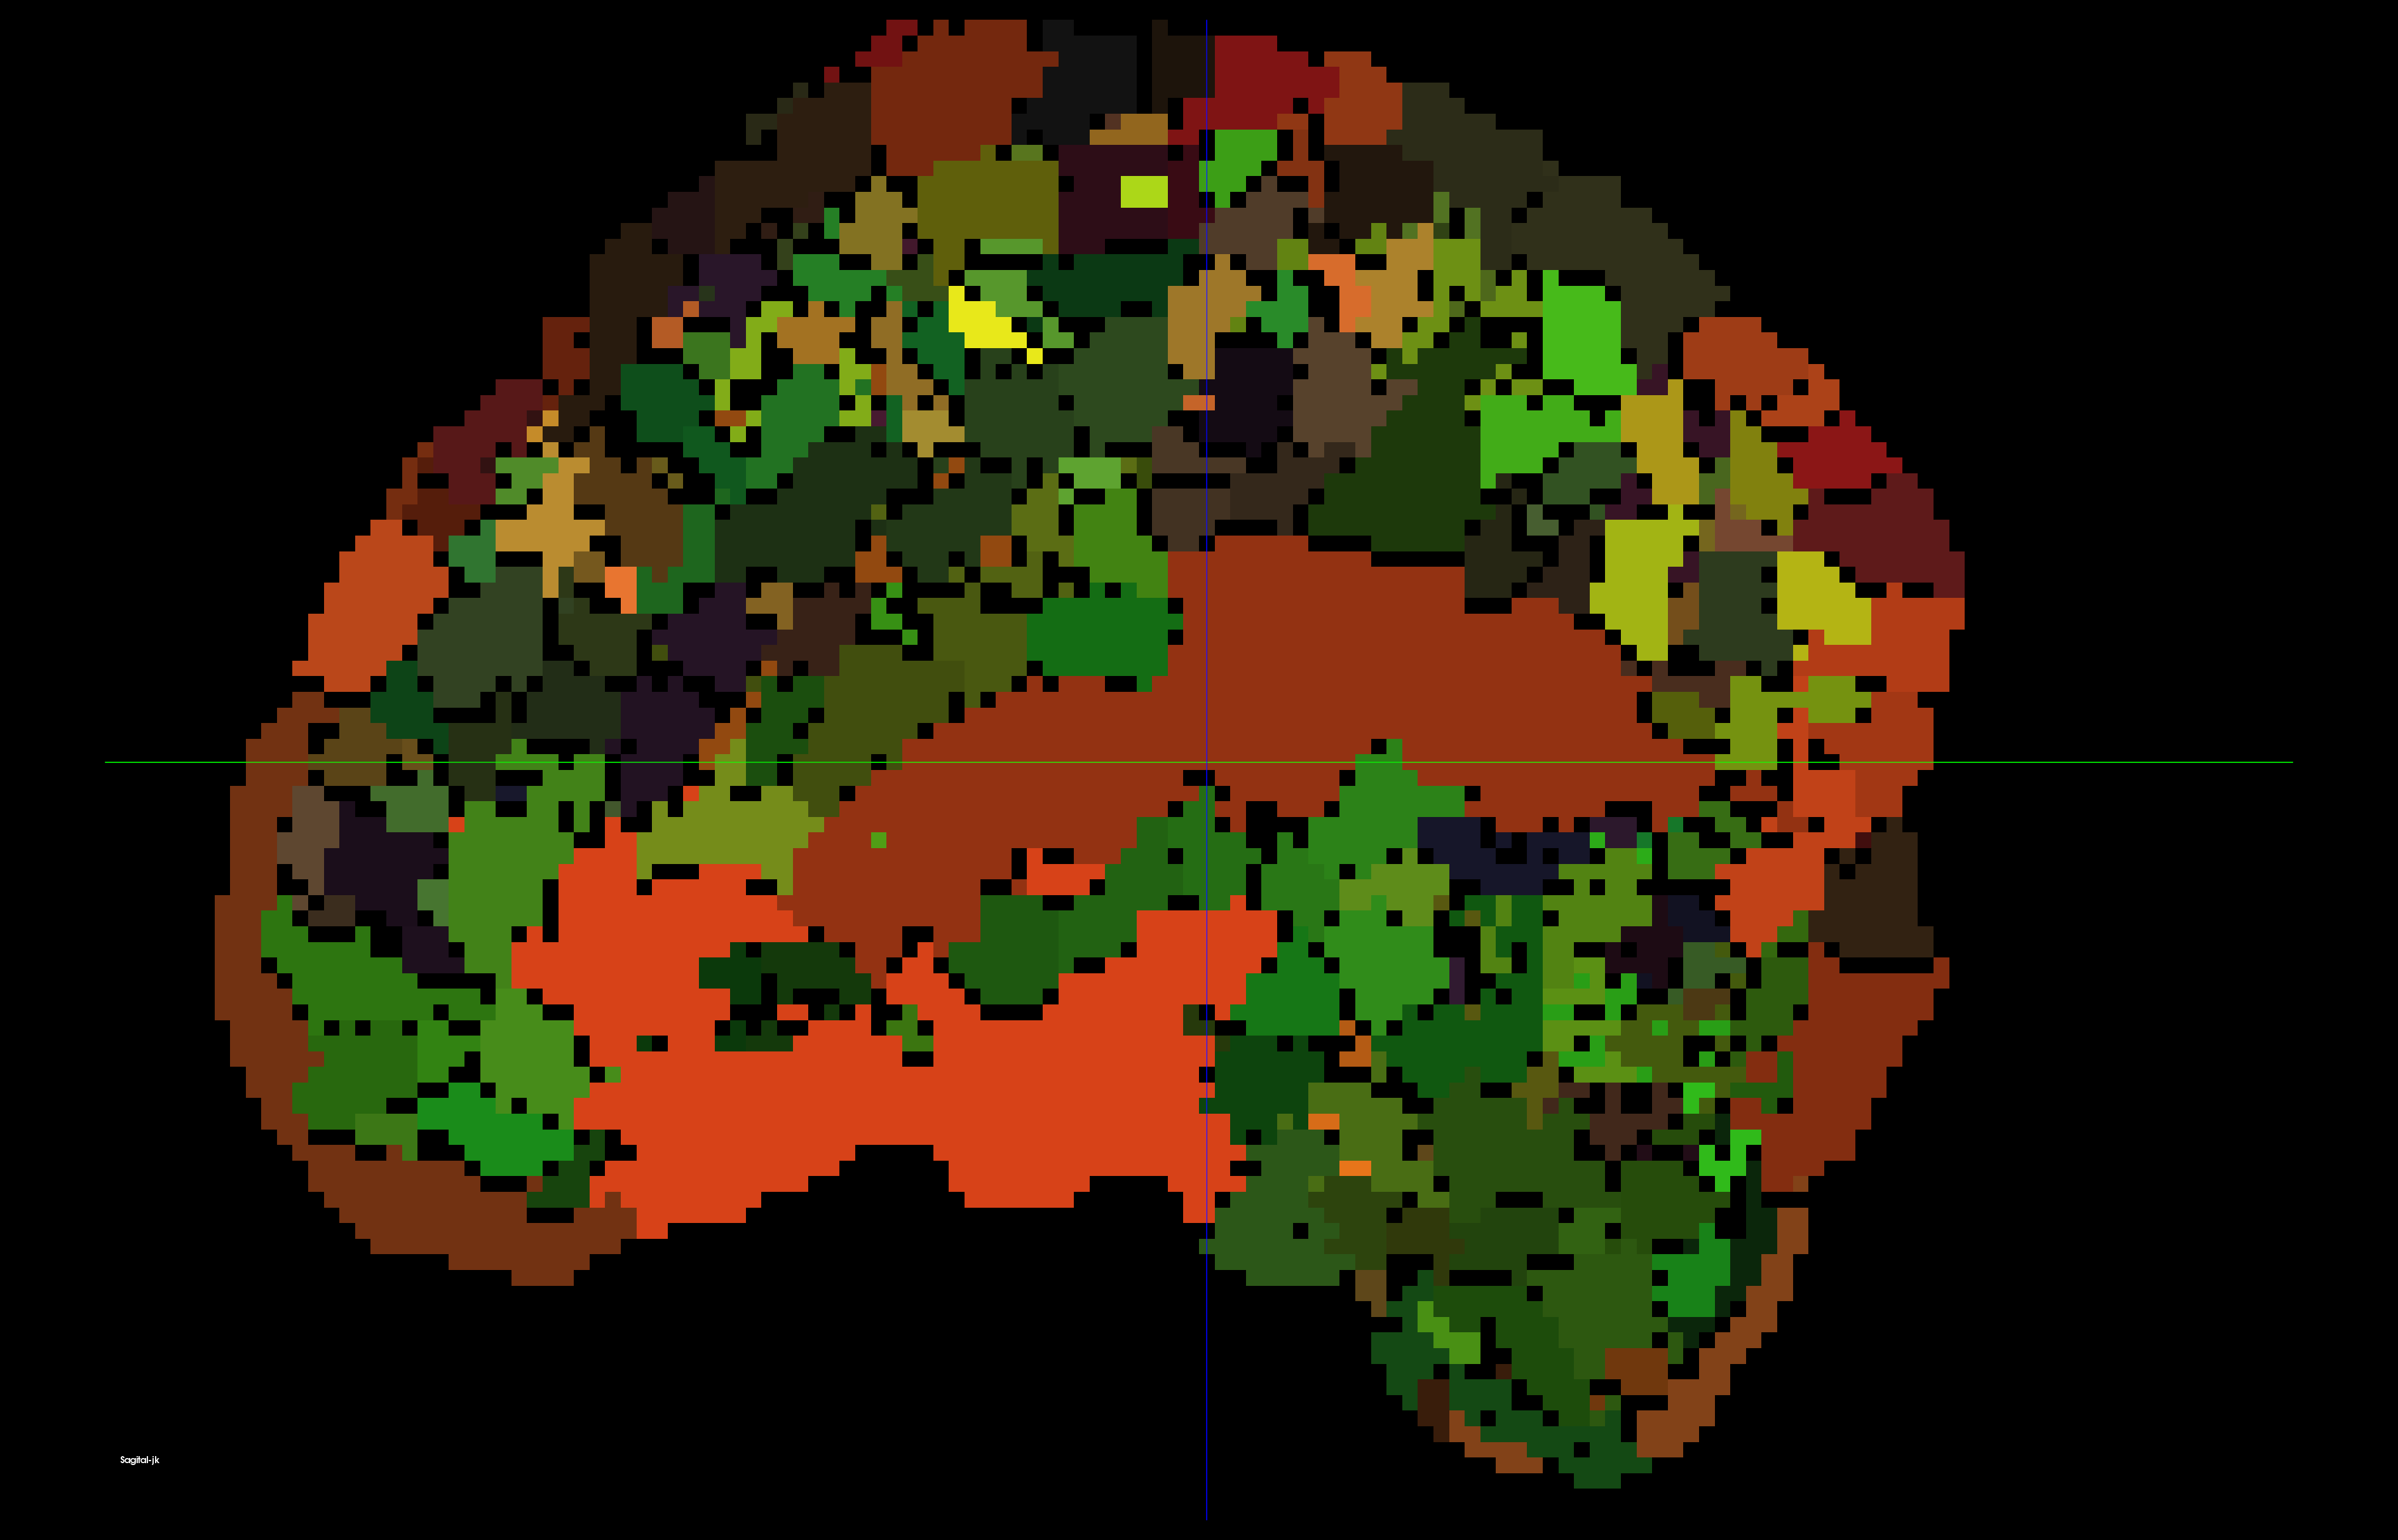
\includegraphics[width=1\linewidth]{imgs/tv_watersheds.png}
      \caption{Sagital cut at (70, 70, 48) for TV watersheds.}
      \label{fig:tv_watersheds}
    \end{figure}

    \subsection{First eigenvalue ($\lambda_1$)}
    \begin{figure}[H]
      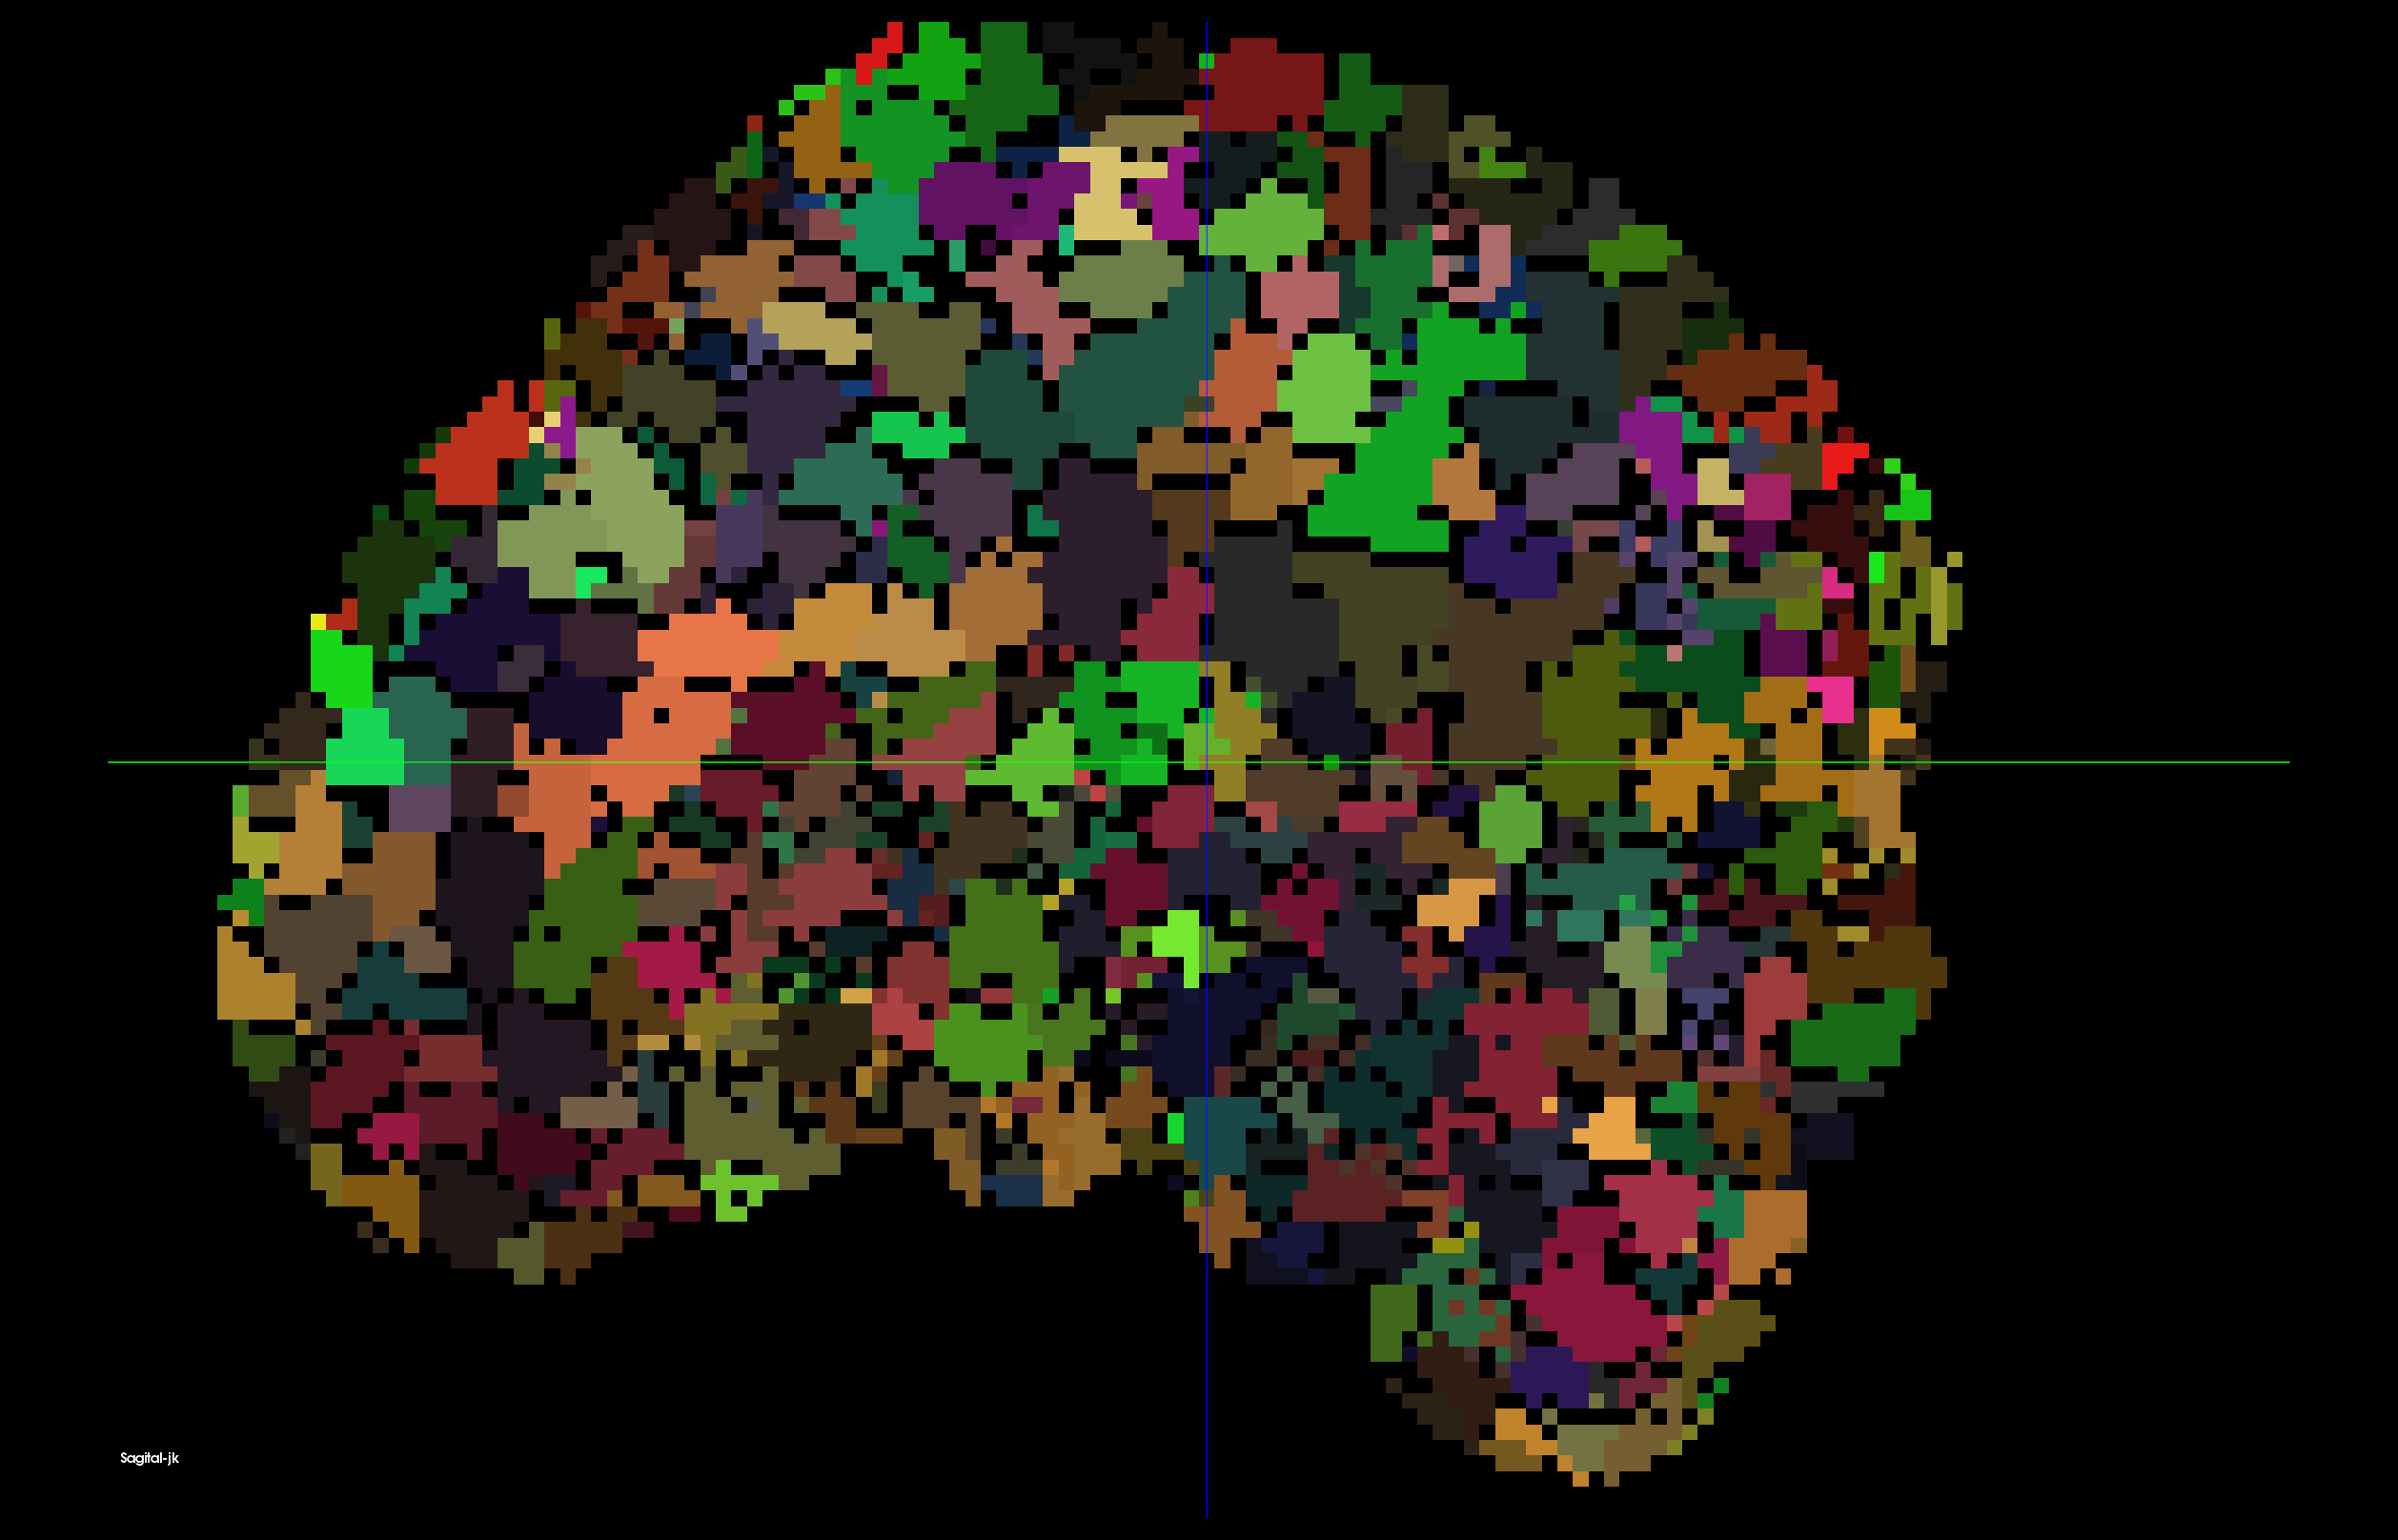
\includegraphics[width=1\linewidth]{imgs/e1_watersheds.png}
      \caption{Sagital cut at (70, 70, 48) for $\lambda_1$ watersheds.}
      \label{fig:e1_watersheds}
    \end{figure}

    \subsection{Second eigenvalue ($\lambda_2$)}
    \begin{figure}[H]
      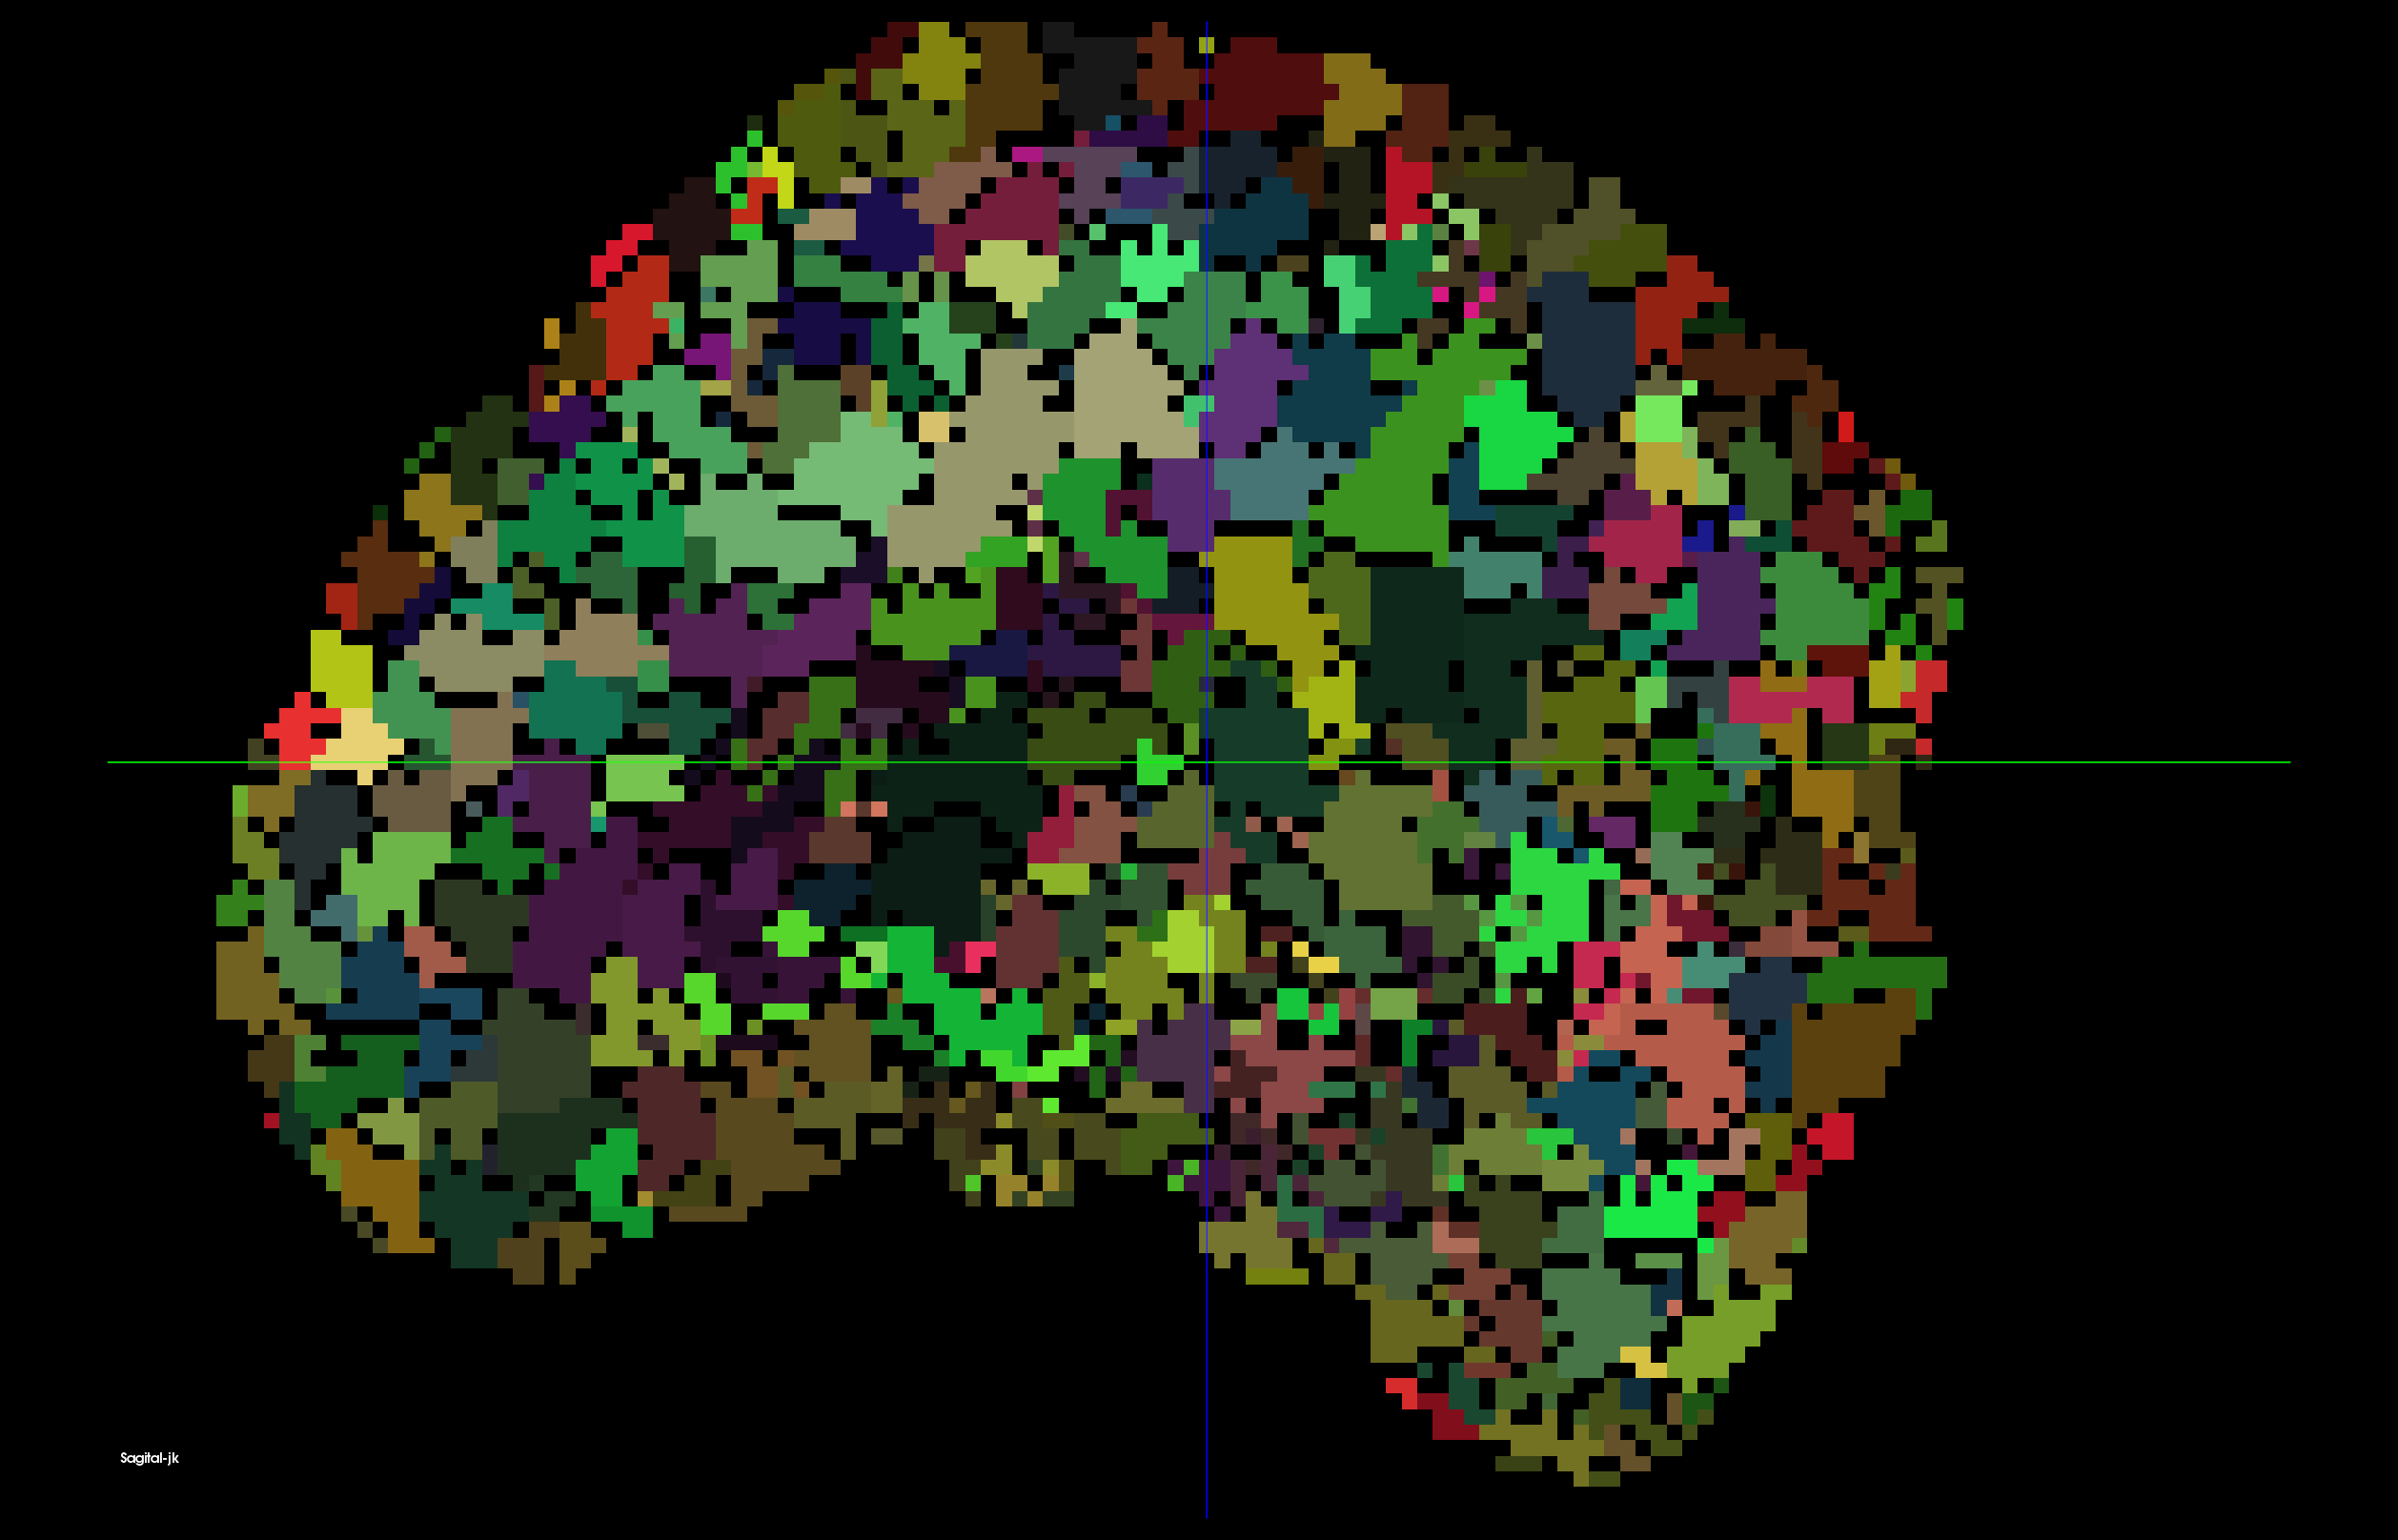
\includegraphics[width=1\linewidth]{imgs/e2_watersheds.png}
      \caption{Sagital cut at (70, 70, 48) for $\lambda_2$ watersheds.}
      \label{fig:e2_watersheds}
    \end{figure}

    \subsection{Third eigenvalue ($\lambda_3$)}
    \begin{figure}[H]
      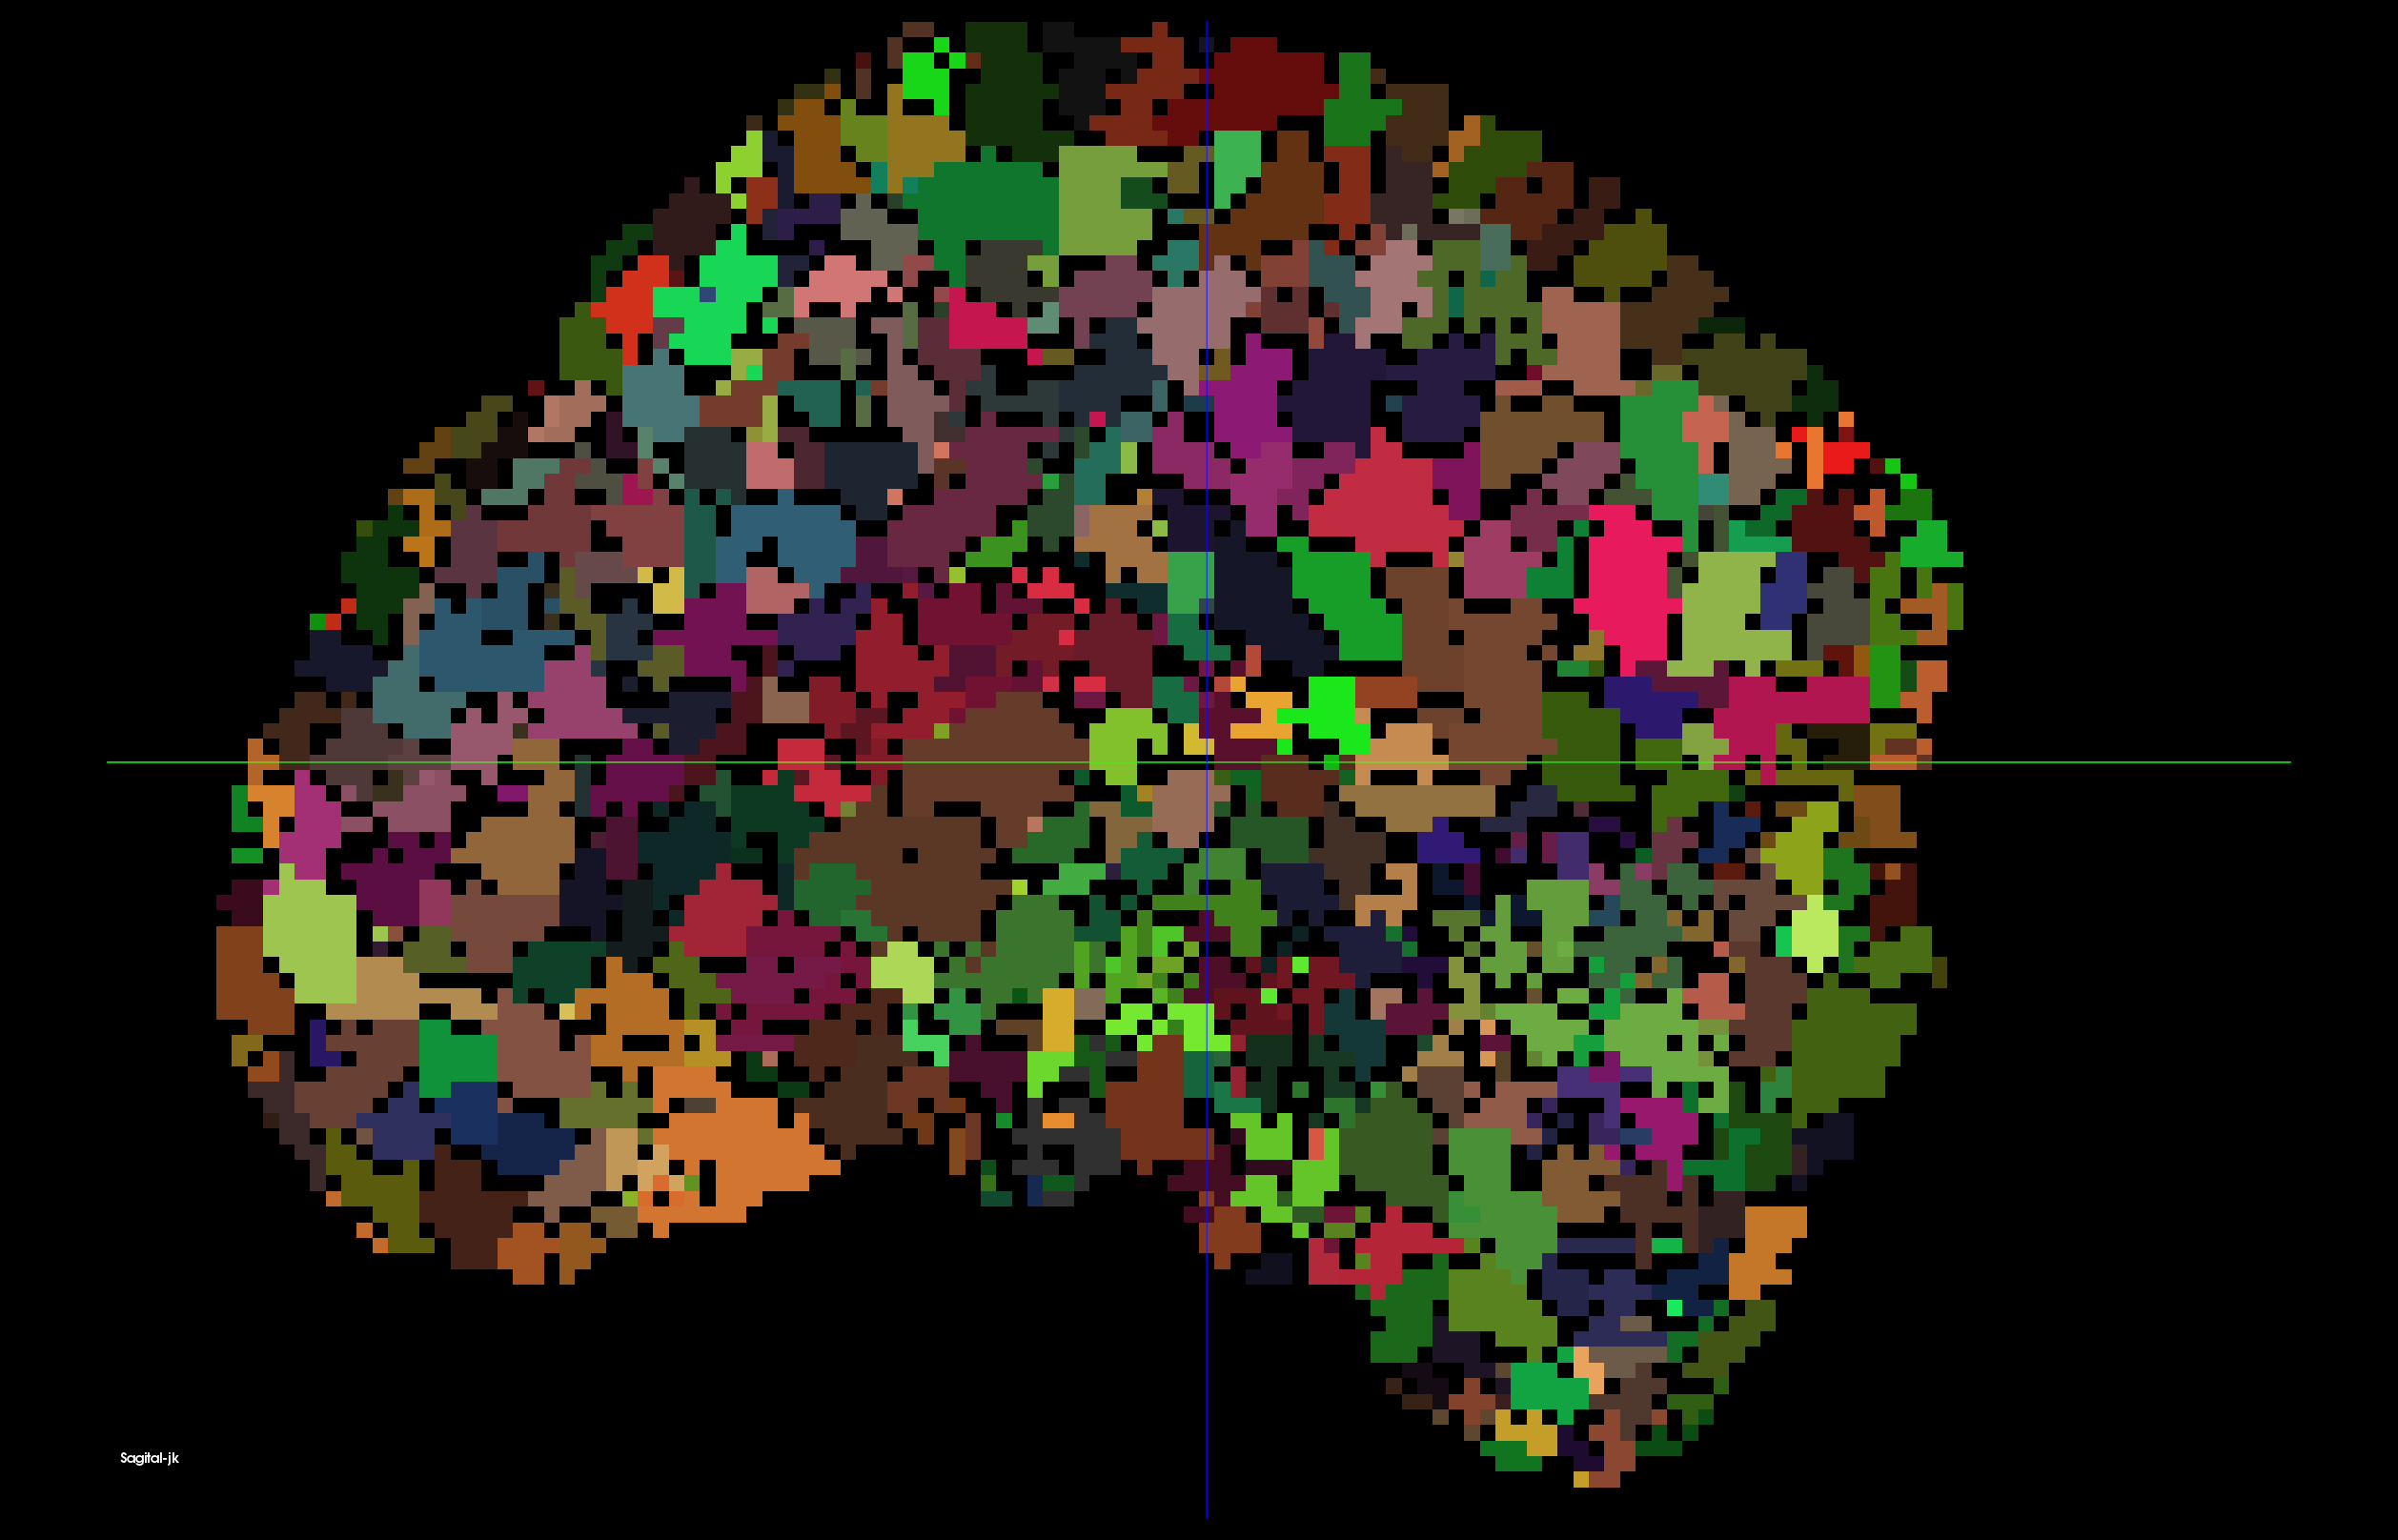
\includegraphics[width=1\linewidth]{imgs/e3_watersheds.png}
      \caption{Sagital cut at (70, 70, 48) for $\lambda_3$ watersheds.}
      \label{fig:e3_watersheds}
    \end{figure}

\chapter{Conclusion}
Finding certainty regions inside a given dataset is easier than finding uncertainty or that there are four or five times more uncertainty regions than certainty.

A second point to take into consideration is that from this results the image segmentation may look like a dead end. But this amount of segmented regions is exactly what is expected from this algorithm on it's article which mentions that it is necessary to apply region growing algorithms after the segmentation in order to obtain meaningful results.

This is a preview of the application of a region grow algorithm to the FA watersheds (\ref{fig:fa_watersheds}):

\begin{figure}[H]
  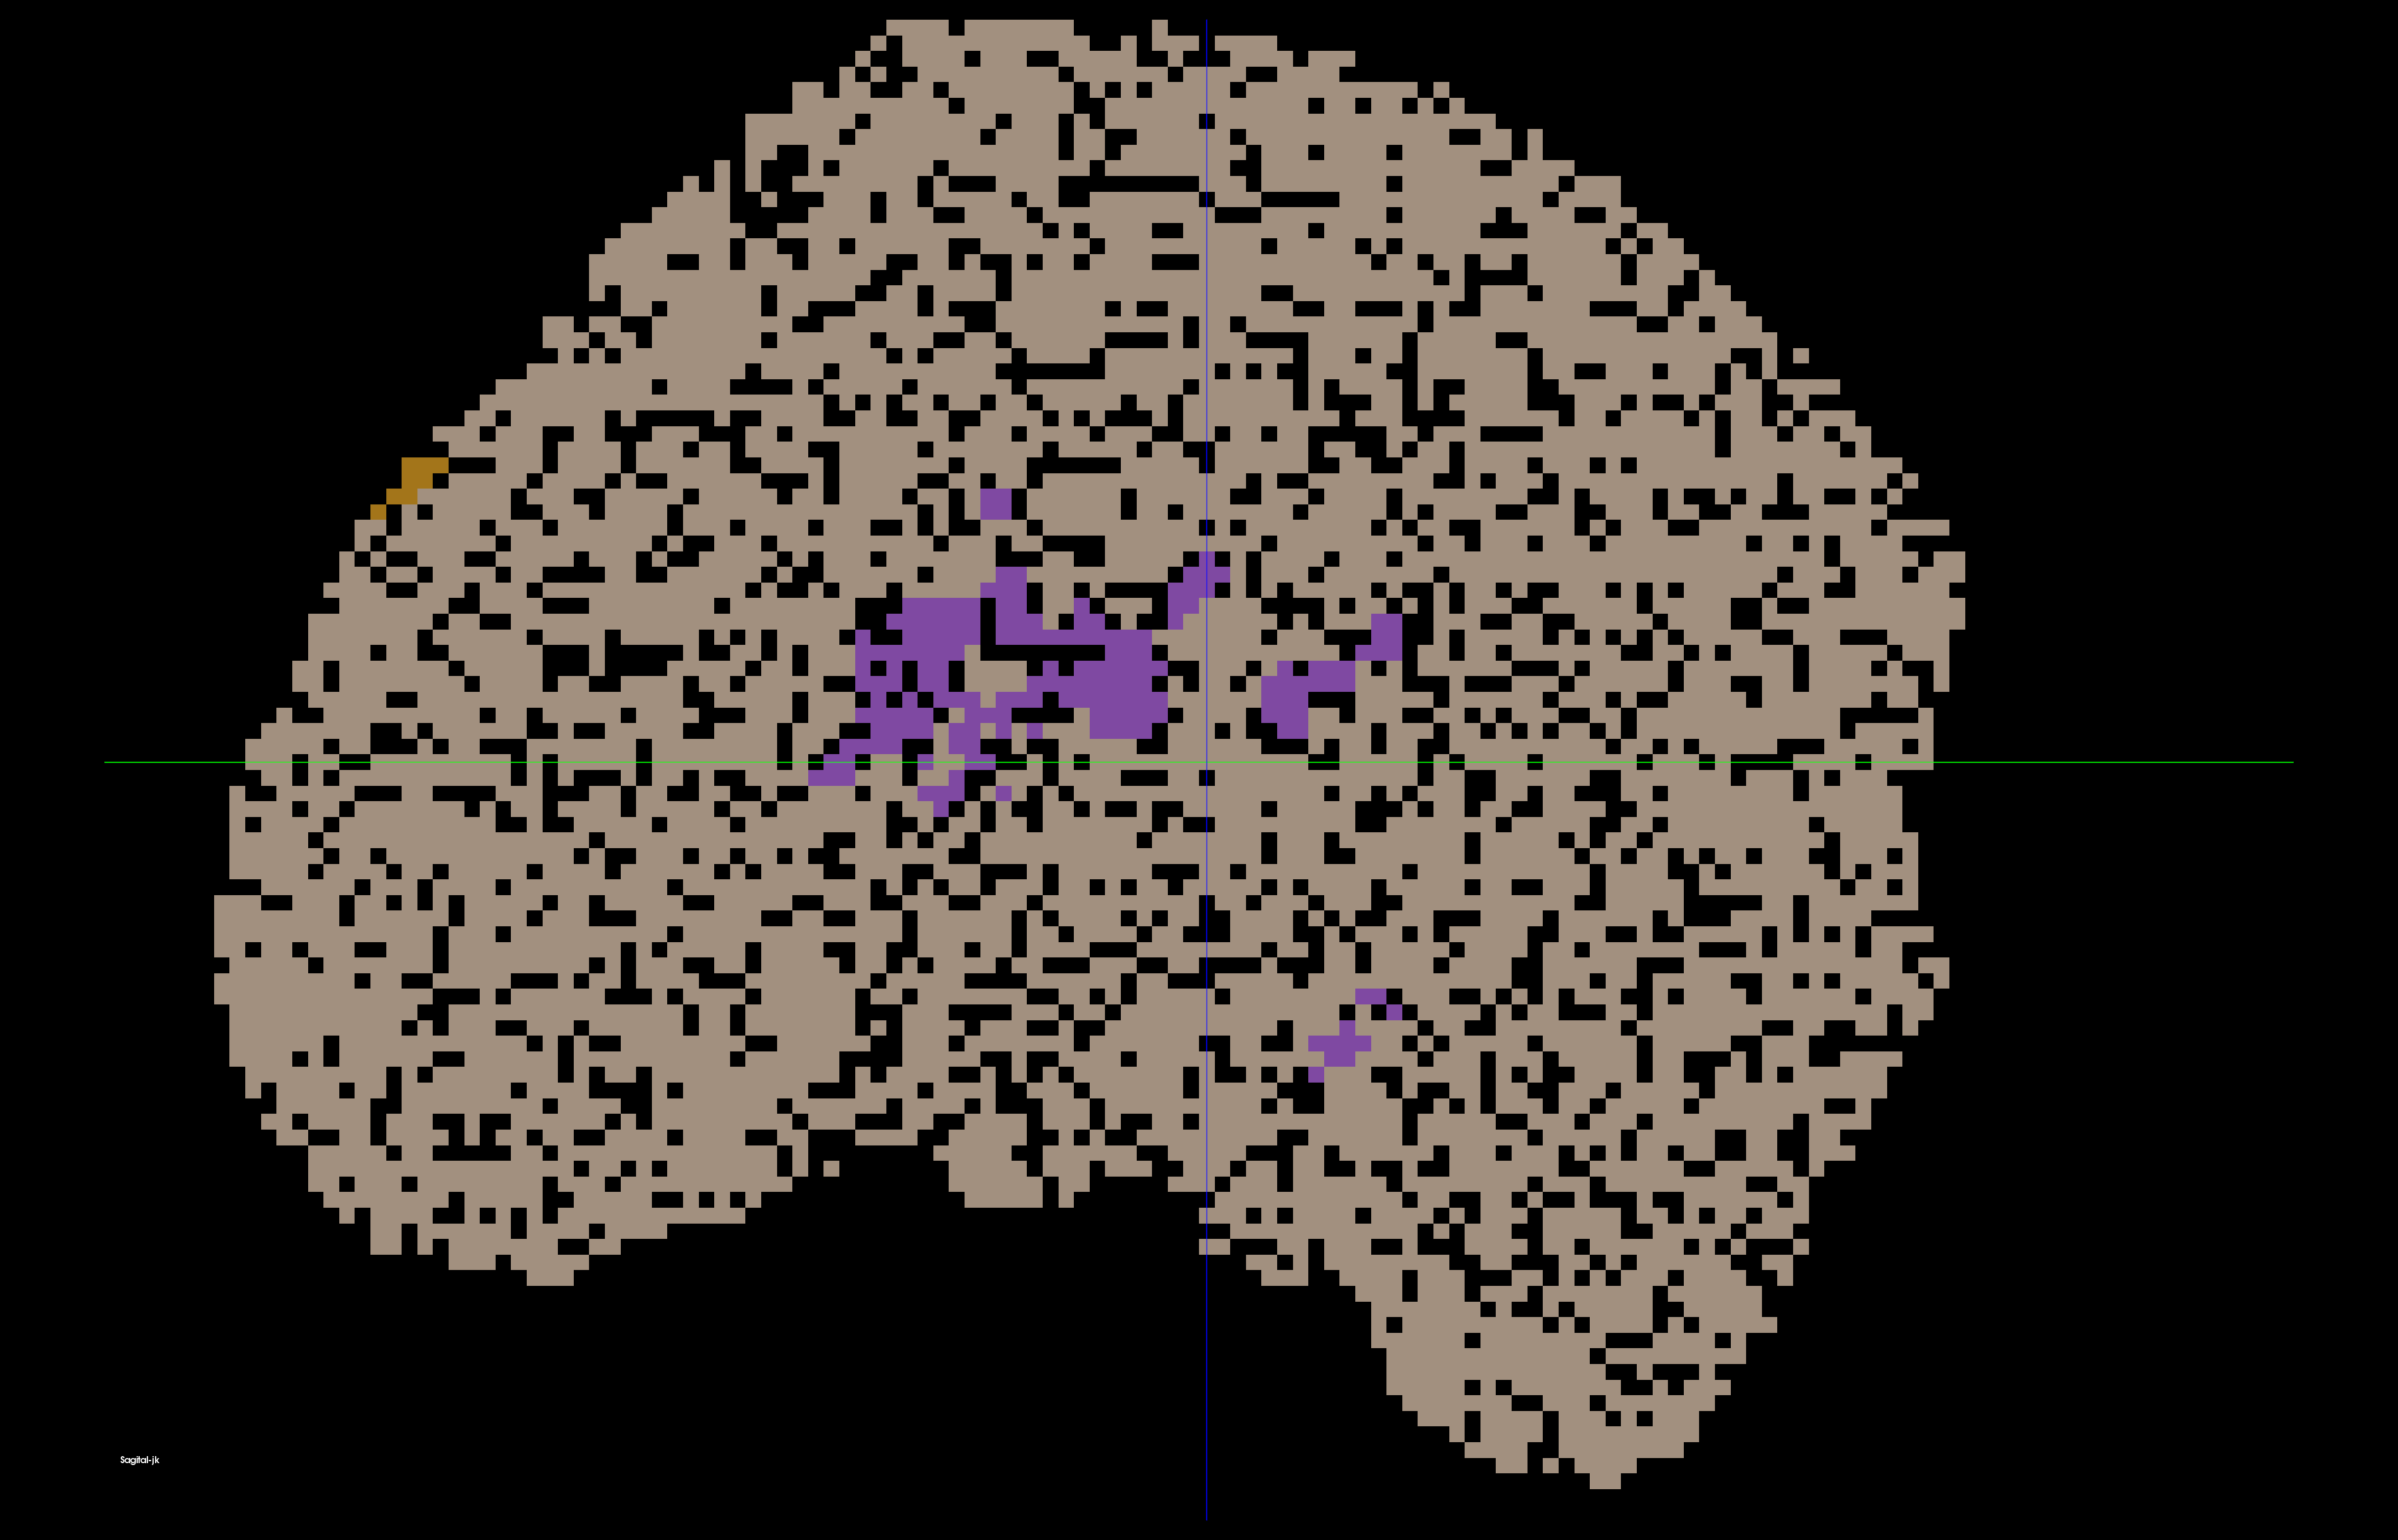
\includegraphics[width=1\linewidth]{imgs/fa_watersheds_01_20_grown.png}
  \caption{Sagital cut at (70, 70, 48) for FA watersheds grown.}
  \label{fig:fa_watersheds_grown}
\end{figure}

Finally one thing that comes to my mind is that, I've mapped 160K voxels as white matter (\ref{fig:fa_threshold}) and that just 40K voxels are certainty regions. Maybe the next step would be to analyse those remaining 120K voxels in detail and apply the region grow watersheds.
\end{document}